\documentclass[landscape]{foils}
\usepackage{graphicx,color,amsmath,amssymb,latexsym,enumerate,rotate,mathabx}
\usepackage{tikz}
\usepackage{changepage}
\usetikzlibrary{arrows,positioning, calc}
\tikzstyle{vertex}=[draw,fill=black!8,circle,minimum size=6pt,inner sep=0pt]

\topmargin-2cm
\leftmargin-1cm
%%\voffset-1.5cm
%%\hoffset.5cm
%\textwidth25cm
%\parindent0pt
\textheight18cm

\MyLogo{Ehrhart Polynomials \quad \includegraphics[viewport= 0 16 100 100, height=16pt]{pentagon} \ Matthias Beck}
\leftheader{}
\rightheader{}

\def\MB{M\hspace{-6pt}B }
\def\mybullet{\green $\blacktriangleright$ \black}

\newcounter{frozenpage}
\def\freezepage{
  \setcounter{frozenpage}{\thepage}
  \renewcommand{\thepage}{\thefrozenpage}
}
\def\thawpage{
  \count0=\thefrozenpage
  \advance\count0by1
  \renewcommand{\thepage}{\the\count0}
}

\definecolor{green}{rgb}{.0,.5,.2}             % green is not always easy to read!
\def\green{\color{green}}
\definecolor{red}{rgb}{.8,.1,.3}
\def\red{\color{red}}
\definecolor{blue}{rgb}{0,0,.7}
\def\blue{\color{blue}}
\def\black{\color{black}}
\def\yellow{\color{yellow}}
\def\cyan{\color{cyan}}
\definecolor{orange}{rgb}{1,.6,0}
\def\orange{\color{orange}}
%\def\magenta{\color{magenta}}

%\def\red{\color{black}}                       % For emergencies 
%\def\green{\color{black}}

\def\bm{\blue $} 
\def\em{$ \black } 
\def\be{\blue \[} 
\def\ee{\] \black}                               % Math mode delimiters
\def\ba{\blue \begin{eqnarray*}} 
\def\ea{\end{eqnarray*} \black}

\def\x{{\boldsymbol x}}
\def\a{{\boldsymbol a}}
\def\b{{\boldsymbol b}}
\def\p{{\boldsymbol p}}
\def\q{{\boldsymbol q}}
\def\c{c}
\DeclareMathOperator{\LH}{LH}

\begin{document}
\setlength{\parindent}{0pt}
\setlength{\parskip}{1cm}

\def\hopen{\mathbb{H}}
\def\Z{\mathbb{Z}}
\def\Q{\mathbb{Q}}
\def\R{\mathbb{R}}
\def\C{\mathcal{C}}
\def\F{\mathcal{F}}
\def\G{\mathcal{G}}
\def\P{\mathcal{P}}
\def\cQ{\mathcal{Q}}
\def\K{\mathcal{K}}
\def\OP{\mathcal{O}}
\def\cZ{\mathcal{Z}}
\def\m{\mathbf{m}}
\def\v{\mathbf{v}}
\def\w{\mathbf{w}}
\def\z{\mathbf{z}}
\newcommand\cone{\operatorname{cone}} 
\newcommand\conv{\operatorname{conv}} 
\newcommand\vol{\operatorname{vol}} 
\newcommand\stir{\operatorname{stirl}}
\newcommand\Ehr{\operatorname{Ehr}} 
\newcommand\fl[1]{\left\lfloor {#1} \right\rfloor} 
\newcommand\fr[1]{\left\{ {#1} \right\}} 
\newcommand\Chat{\widehat{\K}}
\newcommand\PPhat{{\widehat{\Pi}}}
\newcommand\Ccheck{\widecheck{\K}}
\newcommand\PPcheck{\widecheck{\Pi}}

\def\headercolor{\green}

%%%%%%%%%%%%%%%%%%%%%%%%%%%%%%%%%%%%%%%%%%%%%%%%%%%%%

\thispagestyle{empty}
\

\begin{center}
  {\green\LARGE \textbf{Ehrhart Polynomials} \\[12pt]
\normalsize
Day I: Appetizers}
\end{center}

\vspace{-.2in}
%\hspace{5.3in}
\includegraphics[totalheight=5in]{../../David/sublattice3-eps-converted-to}

\vspace{-4.5in} 
\blue
\hspace{5in}
Matthias Beck
\\[5pt]
\black
\hspace{5in}
San Francisco State University
\\[5pt]
\blue
\hspace{5in}
https://matthbeck.github.io/
\black

\vspace{1in} 
\hspace{5in}
VIII Encuentro Colombiano 

\vspace{-.4in} 
\hspace{5in}
De Combinatoria

\black

%%%%%%%%%%%%%%%%%%%%%%%%%%%%%%%%%%%%%%%%%%%%%%%%%%%%%
\newpage
\[  \] 

\vspace{1.5cm} 

``Science is what we understand well enough to explain to a computer, art is all the rest." \\ 

\blue       
Donald Knuth 
\black 

\vspace{-.7in}
\hspace{5in}
\includegraphics[totalheight=3.5in]{../../David/trunccube_arrows-eps-converted-to}

%%%%%%%%%%%%%%%%%%%%%%%%%%%%%%%%%%%%%%%%%%%%%%%%%%%%%

\foilhead[-0pt]{\green Themes}

\blue
\begin{center}
Discrete-geometric \\ polynomials

\vspace{1in}
Generating \\ functions

\vspace{1in}
Polyhedra
\end{center}

\black
\vspace{-1.8in}
Combinatorial \\ structures

\vspace{-3.8in}
\hspace{7in}
Computation 

\vspace{-.4in}
\hspace{7in}
(complexity)

\vspace{-2.2in}
\hspace{-.7in}
\includegraphics[totalheight=2.8in]{../../David/permutahedron4-eps-converted-to}

\vspace{-.1in}
\hspace{6.2in}
\includegraphics[totalheight=3in]{../../David/titlepicturenolables-eps-converted-to}

%%%%%%%%%%%%%%%%%%%%%%%%%%%%%%%%%%%%%%%%%%%%%%%%%%%%%

\foilhead[-40pt]{\green A Sample Problem: Birkhoff--von Neumann Polytope}

\hspace{-.3in}
\includegraphics[totalheight=4.8in]{../oeis}

\vspace{-.7in}
\be B_n \, = \, \left\{ \left( \begin{array}{ccc} x_{11} & \cdots & x_{1n} \\ \vdots & & \vdots \\ x_{n1} & \dots & x_{nn} \end{array} \right) \in \R_{ \geq 0 }^{n^2} \, : \, \begin{array}{l} \sum_j x_{jk} = 1 \text{ for all } 1 \leq k \leq n \\ \sum_k x_{jk} = 1 \text{ for all } 1 \leq j \leq n \end{array} \right\}  \ee 

%%%%%%%%%%%%%%%%%%%%%%%%%%%%%%%%%%%%%%%%%%%%%%%%%%%%%

\foilhead[-20pt]{\green Discrete Volumes}

\red Rational polyhedron \bm \P \subset \R^d \em -- solution set of a system of linear equalities \& inequalities with integer coefficients

\green Goal: \black understand \bm \P \cap \Z^d \em \dots

\vspace{-1in}
\hspace{6.3in}
\includegraphics[totalheight=2in]{../../David/preface_disc-eps-converted-to}

\vspace{-1.5in}
\begin{enumerate}[\mybullet]
\item (list) \bm \displaystyle \sum_{ \m \in \P \cap \Z^d } z_1^{ m_1 } z_2^{ m_2 } \cdots z_d^{ m_d } \em
\item (count) \ \bm \left| \P \cap \Z^d \right| \em
\item (volume) \ \bm \displaystyle \vol(\P) \, = \, \lim_{ t \to \infty } \frac{ 1 }{ t^d } \left| \P \cap \frac 1 t \Z^d \right| \em
\end{enumerate}

\vspace{-2in}
\hspace{6.3in}
\includegraphics[totalheight=2in]{../../David/preface_cont-eps-converted-to}

\freezepage
%%%%%%%%%%%%%%%%%%%%%%%%%%%%%%%%%%%%%%%%%%%%%%%%%%%%%

\foilhead[-20pt]{\green Discrete Volumes}

\red Rational polyhedron \bm \P \subset \R^d \em -- solution set of a system of linear equalities \& inequalities with integer coefficients

\green Goal: \black understand \bm \P \cap \Z^d \em \dots

\vspace{-1in}
\hspace{6.3in}
\includegraphics[totalheight=2in]{../../David/preface_disc-eps-converted-to}

\vspace{-1.5in}
\begin{enumerate}[\mybullet]
\item (list) \bm \displaystyle \sum_{ \m \in \P \cap \Z^d } z_1^{ m_1 } z_2^{ m_2 } \cdots z_d^{ m_d } \em
\item (count) \ \bm \left| \P \cap \Z^d \right| \em
\item (volume) \ \bm \displaystyle \vol(\P) \, = \, \lim_{ t \to \infty } \frac{ 1 }{ t^d } \left| \P \cap \frac 1 t \Z^d \right| \em
\end{enumerate}

\vspace{-2in}
\hspace{6.3in}
\includegraphics[totalheight=2in]{../../David/preface_cont-eps-converted-to}

\vspace{-.2in}
\red Ehrhart function \ \bm \displaystyle L_\P (t) \, := \, \left| \P \cap \frac 1 t \Z^d \right| \, = \, \left| t \P \cap \Z^d \right| \em \ for \bm t \in \Z_{ >0 } \em

%%%%%%%%%%%%%%%%%%%%%%%%%%%%%%%%%%%%%%%%%%%%%%%%%%%%%

\foilhead[-20pt]{\green Some Motivation}

\begin{enumerate}[\mybullet]
\item Linear systems are \blue everywhere \black \!\!, and so polyhedra are everywhere.
\end{enumerate}

\thawpage
\freezepage
%%%%%%%%%%%%%%%%%%%%%%%%%%%%%%%%%%%%%%%%%%%%%%%%%%%%%

\foilhead[-20pt]{\green Some Motivation}

\begin{enumerate}[\mybullet]
\item Linear systems are \blue everywhere \black \!\!, and so polyhedra are everywhere.
\item In applications, the \blue volume \black of the polytope represented by a linear system measures some fundamental data of this system (``average").
\end{enumerate}

%%%%%%%%%%%%%%%%%%%%%%%%%%%%%%%%%%%%%%%%%%%%%%%%%%%%%

\foilhead[-20pt]{\green Some Motivation}

\begin{enumerate}[\mybullet]
\item Linear systems are \blue everywhere \black \!\!, and so polyhedra are everywhere.
\item In applications, the \blue volume \black of the polytope represented by a linear system measures some fundamental data of this system (``average").
\item Many \blue discrete problems \black in various areas are linear problems, thus they ask for the discrete volume of a polytope in disguise.
\end{enumerate}

%%%%%%%%%%%%%%%%%%%%%%%%%%%%%%%%%%%%%%%%%%%%%%%%%%%%%

\foilhead[-20pt]{\green Some Motivation}

\begin{enumerate}[\mybullet]
\item Linear systems are \blue everywhere \black \!\!, and so polyhedra are everywhere.
\item In applications, the \blue volume \black of the polytope represented by a linear system measures some fundamental data of this system (``average").
\item Many \blue discrete problems \black in various areas are linear problems, thus they ask for the discrete volume of a polytope in disguise.
\item Much discrete geometry can be modeled using \blue polynomials \black and, conversely, many combinatorial polynomials can be modeled geometrically.
\end{enumerate}

%%%%%%%%%%%%%%%%%%%%%%%%%%%%%%%%%%%%%%%%%%%%%%%%%%%%%

\foilhead[-20pt]{\green Some Motivation}

\begin{enumerate}[\mybullet]
\item Linear systems are \blue everywhere \black \!\!, and so polyhedra are everywhere.
\item In applications, the \blue volume \black of the polytope represented by a linear system measures some fundamental data of this system (``average").
\item Many \blue discrete problems \black in various areas are linear problems, thus they ask for the discrete volume of a polytope in disguise.
\item Much discrete geometry can be modeled using \blue polynomials \black and, conversely, many combinatorial polynomials can be modeled geometrically.
\item Polytopes are basic geometric objects, yet even for these basic objects volume computation is \blue hard \black and there remain many open problems.
\end{enumerate}

%%%%%%%%%%%%%%%%%%%%%%%%%%%%%%%%%%%%%%%%%%%%%%%%%%%%%

\foilhead[-20pt]{\green Some Motivation}

\begin{enumerate}[\mybullet]
\item Linear systems are \blue everywhere \black \!\!, and so polyhedra are everywhere.
\item In applications, the \blue volume \black of the polytope represented by a linear system measures some fundamental data of this system (``average").
\item Many \blue discrete problems \black in various areas are linear problems, thus they ask for the discrete volume of a polytope in disguise.
\item Much discrete geometry can be modeled using \blue polynomials \black and, conversely, many combinatorial polynomials can be modeled geometrically.
\item Polytopes are basic geometric objects, yet even for these basic objects volume computation is \blue hard \black and there remain many open problems.
\item Also, polytopes are \blue cool \black\!\!.
\end{enumerate}

%%%%%%%%%%%%%%%%%%%%%%%%%%%%%%%%%%%%%%%%%%%%%%%%%%%%%

\foilhead{\green Today's Menu: Get Our Hands Dirty}

\vspace{-.3in}
\hspace{2.3in}
\includegraphics[totalheight=3in]{../../David/cube-eps-converted-to}

\vspace{-1.6in}
%\hspace{3in}
%\includegraphics[totalheight=3in]{../../David/standsimplex-eps-converted-to}
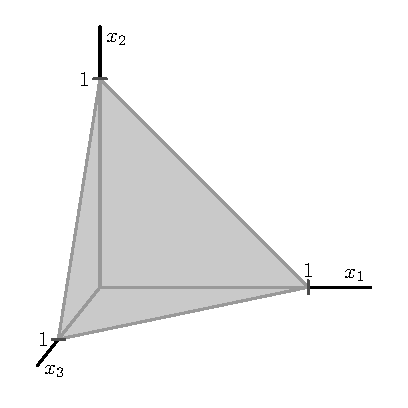
\includegraphics[totalheight=4in]{../../David/fig22c}

\vspace{-4.3in}
\hspace{5in}
\includegraphics[totalheight=4.2in]{../../David/octahedron-eps-converted-to}

\thawpage
%%%%%%%%%%%%%%%%%%%%%%%%%%%%%%%%%%%%%%%%%%%%%%%%%%%%%

\foilhead[-20pt]{\green The Unit Cube}

\red Lattice polytope \bm \P \subset \R^d \em -- convex hull of finitely points in \bm \Z^d \em

For \bm t \in \Z_{ >0 } \em let \bm L_\P (t) \, := \, \# \left( t \P \cap \Z^d \right) \em

The \red unit cube \black in \bm \R^d \em is
\ \bm \P \, = \, [0,1]^d \, = \, \left\{ \x \in \R^d : \, 0 \le x_j \le 1 \right\}  \em

\vspace{.1in}
%\hspace{4.3in}
\includegraphics[totalheight=3.4in]{../../David/cube-eps-converted-to}

\vspace{-3.3in}
\hspace{4.3in}
\green $\longrightarrow$ \ \bm L_\P(t) \, = \, (t+1)^d \em

\freezepage
%%%%%%%%%%%%%%%%%%%%%%%%%%%%%%%%%%%%%%%%%%%%%%%%%%%%%

\foilhead[-20pt]{\green The Unit Cube}

\red Lattice polytope \bm \P \subset \R^d \em -- convex hull of finitely points in \bm \Z^d \em

For \bm t \in \Z_{ >0 } \em let \bm L_\P (t) \, := \, \# \left( t \P \cap \Z^d \right) \em

The \red unit cube \black in \bm \R^d \em is
\ \bm \P \, = \, [0,1]^d \, = \, \left\{ \x \in \R^d : \, 0 \le x_j \le 1 \right\}  \em

\vspace{.1in}
%\hspace{4.3in}
\includegraphics[totalheight=3.4in]{../../David/cube-eps-converted-to}

\vspace{-3.3in}
\hspace{4.3in}
\green $\longrightarrow$ \ \bm L_\P(t) \, = \, (t+1)^d \em

\vspace{.6in}
\hspace{4.82in}
\green \bm L_{\P^\circ}(t) \, = \, (t-1)^d \em

%%%%%%%%%%%%%%%%%%%%%%%%%%%%%%%%%%%%%%%%%%%%%%%%%%%%%

\foilhead[-20pt]{\green The Standard Simplex}

The \red standard simplex \bm \Delta \in \R^d \em is the convex hull of the
unit vectors and the origin; alternatively,

\vspace{.3in}
\hspace{2.9in}
\bm
\Delta \ = \ \left\{ \x \in \R_{ \ge 0 }^d : \, x_1 + x_2 + \cdots + x_d \le 1 \right\}
\em

\vspace{-.6in}
%\hspace{.3in}
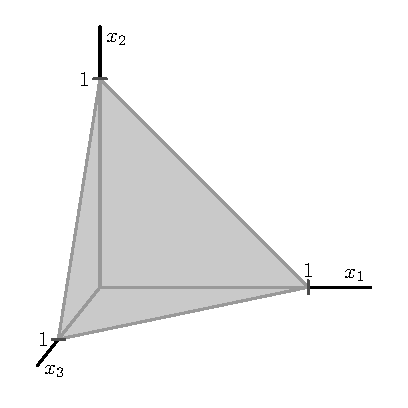
\includegraphics[totalheight=4in]{../../David/fig22c}

\thawpage
\freezepage
%%%%%%%%%%%%%%%%%%%%%%%%%%%%%%%%%%%%%%%%%%%%%%%%%%%%%

\foilhead[-20pt]{\green The Standard Simplex}

The \red standard simplex \bm \Delta \in \R^d \em is the convex hull of the
unit vectors and the origin; alternatively,
\be
\Delta \ = \ \left\{ \x \in \R_{ \ge 0 }^d : \, x_1 + x_2 + \cdots + x_d \le 1 \right\}
\ee

\vspace{-1in}
\ba
L_\Delta(t) 
&=& \# \left\{ (x_1, x_2 \dots, x_d) \in \Z_{ \ge 0 }^d : \, x_1 + x_2 + \cdots + x_d \le t \right\} \\
&=& \# \left\{ (x_1, x_2 \dots, x_d, x_{ d+1 } ) \in \Z_{ \ge 0 }^{d+1} : \, x_1 +
x_2 + \cdots + x_{ d+1 } = t \right\} \\
&=& \binom{ d+t } d
\ea

%%%%%%%%%%%%%%%%%%%%%%%%%%%%%%%%%%%%%%%%%%%%%%%%%%%%%

\foilhead[-20pt]{\green The Standard Simplex}

The \red standard simplex \bm \Delta \in \R^d \em is the convex hull of the
unit vectors and the origin; alternatively,
\be
\Delta \ = \ \left\{ \x \in \R_{ \ge 0 }^d : \, x_1 + x_2 + \cdots + x_d \le 1 \right\}
\ee

\vspace{-1in}
\ba
L_\Delta(t) 
&=& \# \left\{ (x_1, x_2 \dots, x_d) \in \Z_{ \ge 0 }^d : \, x_1 + x_2 + \cdots + x_d \le t \right\} \\
&=& \# \left\{ (x_1, x_2 \dots, x_d, x_{ d+1 } ) \in \Z_{ \ge 0 }^{d+1} : \, x_1 +
x_2 + \cdots + x_{ d+1 } = t \right\} \\
&=& \binom{ d+t } d
\ea

\vspace{-.2in}
\bm \displaystyle
L_{ \Delta^\circ } (t) \ = \ \binom{t-1} d 
\em

%%%%%%%%%%%%%%%%%%%%%%%%%%%%%%%%%%%%%%%%%%%%%%%%%%%%%

\foilhead[-20pt]{\green The Cross-Polytope}

The \red cross-polytope \bm \Diamond \in \R^d \em is

\bm
\Diamond \ = \ \left\{ \x \in \R^d : \, \left| x_1 \right| + \left| x_2 \right| + \dots + \left| x_d \right| \leq 1 \right\}
\em

\vspace{-1.7in}
\hspace{5in}
\includegraphics[totalheight=3.9in]{../../David/octahedron-eps-converted-to}

\thawpage
\freezepage
%%%%%%%%%%%%%%%%%%%%%%%%%%%%%%%%%%%%%%%%%%%%%%%%%%%%%

\foilhead[-20pt]{\green The Cross-Polytope}

The \red cross-polytope \bm \Diamond \in \R^d \em is

\bm
\Diamond \ = \ \left\{ \x \in \R^d : \, \left| x_1 \right| + \left| x_2 \right| + \dots + \left| x_d \right| \leq 1 \right\}
\em

\vspace{-1.7in}
\hspace{5in}
\includegraphics[totalheight=3.9in]{../../David/octahedron-eps-converted-to}

\vspace{-2.3in}
Let's compute \bm L_\Diamond(t) \em for \bm d=3 \em \dots

\vspace{.2in}
\begin{enumerate}[\mybullet]
\item Triangulation
\item Disjoint triangulation
\item Interpolation
\item Generating function
\end{enumerate}

%%%%%%%%%%%%%%%%%%%%%%%%%%%%%%%%%%%%%%%%%%%%%%%%%%%%%

\foilhead[-20pt]{\green The Cross-Polytope}

The \red cross-polytope \bm \Diamond \in \R^d \em is

\bm
\Diamond \ = \ \left\{ \x \in \R^d : \, \left| x_1 \right| + \left| x_2 \right| + \dots + \left| x_d \right| \leq 1 \right\}
\em

\vspace{-1.7in}
\hspace{5in}
\includegraphics[totalheight=3.9in]{../../David/octahedron-eps-converted-to}

\vspace{-2.3in}
Let's compute \bm L_\Diamond(t) \em for \bm d=3 \em \dots

\vspace{.2in}
\begin{enumerate}[\mybullet]
\item Triangulation
\end{enumerate}

Dissect \bm \Diamond \em into \bm 8 \em (standard) tetrahedra and use
inclusion--exclusion to compute \bm L_\Diamond(t) \em

%%%%%%%%%%%%%%%%%%%%%%%%%%%%%%%%%%%%%%%%%%%%%%%%%%%%%

\foilhead[-20pt]{\green The Cross-Polytope}

The \red cross-polytope \bm \Diamond \in \R^d \em is

\bm
\Diamond \ = \ \left\{ \x \in \R^d : \, \left| x_1 \right| + \left| x_2 \right| + \dots + \left| x_d \right| \leq 1 \right\}
\em

\vspace{-1.7in}
\hspace{5in}
\includegraphics[totalheight=3.9in]{../../David/octahedron-eps-converted-to}

\vspace{-2.3in}
Let's compute \bm L_\Diamond(t) \em for \bm d=3 \em \dots

\vspace{.2in}
\begin{enumerate}[\mybullet]
\item Disjoint triangulation
\end{enumerate}

Dissect \bm \Diamond \em into \bm 8 \em half-open tetrahedra 

%%%%%%%%%%%%%%%%%%%%%%%%%%%%%%%%%%%%%%%%%%%%%%%%%%%%%

\foilhead[-20pt]{\green The Cross-Polytope}

The \red cross-polytope \bm \Diamond \in \R^d \em is

\bm
\Diamond \ = \ \left\{ \x \in \R^d : \, \left| x_1 \right| + \left| x_2 \right| + \dots + \left| x_d \right| \leq 1 \right\}
\em

\vspace{-1.7in}
\hspace{5in}
\includegraphics[totalheight=3.9in]{../../David/octahedron-eps-converted-to}

\vspace{-2.3in}
Let's compute \bm L_\Diamond(t) \em for \bm d=3 \em \dots

\vspace{-.1in}
\begin{enumerate}[\mybullet]
\item Interpolation
\end{enumerate}

\vspace{-.1in}
%\hspace{2.3in}
\includegraphics[totalheight=2.3in]{interpol}

% V = matrix.vandermonde([1,2,3,4])

\thawpage
%%%%%%%%%%%%%%%%%%%%%%%%%%%%%%%%%%%%%%%%%%%%%%%%%%%%%

\foilhead[-20pt]{\green The Cross-Polytope}

The \red cross-polytope \bm \Diamond \in \R^d \em is

\bm
\Diamond \ = \ \left\{ \x \in \R^d : \, \left| x_1 \right| + \left| x_2 \right| + \dots + \left| x_d \right| \leq 1 \right\}
\em

\vspace{-1.7in}
\hspace{5in}
\includegraphics[totalheight=3.9in]{../../David/octahedron-eps-converted-to}

\vspace{-2.3in}
Let's compute \bm L_\Diamond(t) \em for \bm d=3 \em \dots

\vspace{.2in}
\begin{enumerate}[\mybullet]
\item Generating function
\end{enumerate}

\vspace{-.4in}
\hspace{1.5in}
\bm \displaystyle \Ehr_\Diamond (z) \, := \, 1 + \sum_{ t \ge 1 } L_\Diamond (t) \, z^t \em 

\freezepage
%%%%%%%%%%%%%%%%%%%%%%%%%%%%%%%%%%%%%%%%%%%%%%%%%%%%%

\foilhead[-20pt]{\green The Cross-Polytope}

The \red cross-polytope \bm \Diamond \in \R^d \em is

\bm
\Diamond \ = \ \left\{ \x \in \R^d : \, \left| x_1 \right| + \left| x_2 \right| + \dots + \left| x_d \right| \leq 1 \right\}
\em

\vspace{-1.7in}
\hspace{5in}
\includegraphics[totalheight=3.9in]{../../David/octahedron-eps-converted-to}

\vspace{-2.3in}
Let's compute \bm L_\Diamond(t) \em for \bm d=3 \em \dots

\vspace{.2in}
\begin{enumerate}[\mybullet]
\item Generating function
\end{enumerate}

\vspace{-.4in}
\hspace{1.5in}
\bm \displaystyle \Ehr_\Diamond (z) \, := \, 1 + \sum_{ t \ge 1 } L_\Diamond (t) \, z^t % \em 
\, = \, \frac{ (1+z)^3 }{ (1-z)^4 } \em

\vspace{-.1in}
Exercise:
\newcommand\DouPyr{\operatorname{BiPyr}} 
\bm \displaystyle
\Ehr_{ \DouPyr (\P) } (z) \ = \ \frac{ 1+z }{ 1-z } \Ehr_\P (z) 
\em

\vspace{.1in}
\hspace{3.5in}
\dots for unit cubes \ \green $\longrightarrow$ \ \black Eulerian polynomials

%%%%%%%%%%%%%%%%%%%%%%%%%%%%%%%%%%%%%%%%%%%%%%%%%%%%%

\foilhead{\green Zonotopes}

\vspace{-1.4in}
\hspace{7in}
\includegraphics[totalheight=2.2in]{../../David/trunccube_arrows-eps-converted-to}

\vspace{-1.4in}
Line segment \
\bm [\a,\b] := \{ (1-\lambda) \, \a + \lambda \, \b : \, 0 \le \lambda \le 1 \} \em

Minkowski sum \
\bm \K_1 + \K_2 \ := \ \{ \p+\q : \, \p \in \K_1, \ \q \in \K_2 \} \em 

\hspace{2.5in}
Zonotope \ \bm \cZ := [\a_1,\b_1] + [\a_2,\b_2] + \cdots + [\a_m,\b_m] \em

\vspace{-.9in}
\includegraphics[totalheight=2.2in]{../../David/zonotopeex-eps-converted-to}

\thawpage
\freezepage
%%%%%%%%%%%%%%%%%%%%%%%%%%%%%%%%%%%%%%%%%%%%%%%%%%%%%

\foilhead{\green Zonotopes}

\vspace{-1.4in}
\hspace{7in}
\includegraphics[totalheight=2.2in]{../../David/trunccube_arrows-eps-converted-to}

\vspace{-1.4in}
Line segment \
\bm [\a,\b] := \{ (1-\lambda) \, \a + \lambda \, \b : \, 0 \le \lambda \le 1 \} \em

Minkowski sum \
\bm \K_1 + \K_2 \ := \ \{ \p+\q : \, \p \in \K_1, \ \q \in \K_2 \} \em 

\hspace{2.5in}
Zonotope \ \bm \cZ := [\a_1,\b_1] + [\a_2,\b_2] + \cdots + [\a_m,\b_m] \em

\vspace{-.9in}
\includegraphics[totalheight=2.2in]{../../David/zonotopeex-eps-converted-to}

\vspace{-1.8in}
\hspace{2.5in}
Every zonotope admits a \red tiling \black into parallelepipeds

\vspace{-.3in}
\hspace{4.1in}
\includegraphics[totalheight=3in]{../../David/zonotopepaving-eps-converted-to}

\vspace{-1.8in}
\bm \P \em --- half-open \bm d \em\!\!-parallelepiped

\green $\longrightarrow$ \ \bm L_\P(t) \, = \, \vol(\P) \, t^d \em

%%%%%%%%%%%%%%%%%%%%%%%%%%%%%%%%%%%%%%%%%%%%%%%%%%%%%

\foilhead{\green Recap Day I}

\vspace{-.2in}
\begin{enumerate}[\mybullet]
\item Volume computations \ \bm \longrightarrow \em \ don't agonize, discretize 
\item Integer-point counting in dilated polytopes \ \bm \longrightarrow \em \
polynomials
\item Interpolation
\item Generating functions
\item Dissections: triangulations, tilings
\item Tomorrow: enough practice, how \\ does this work in theory?
\end{enumerate}

\vspace{-3.2in}
\hspace{5.7in}
\includegraphics[totalheight=3.7in]{beckcycle}

\vspace{-3in}
\hspace{8.4in}
\tiny
\rotatebox{90}{\copyright Math 883 (2022)}

\normalsize

\thawpage
%%%%%%%%%%%%%%%%%%%%%%%%%%%%%%%%%%%%%%%%%%%%%%%%%%%%%

\foilhead{\green Birkhoff--von Neumann Revisited}

\vspace{-.7in}
\includegraphics[totalheight=5.8in]{../birkhoff9roots}

\vspace{-4.5in}
\hspace{5in}
For more about roots of 

\vspace{-.35in}
\hspace{5in}
(Ehrhart) polynomials, 

\vspace{-.35in}
\hspace{5in}
see Braun (2008) and 

\vspace{-.35in}
\hspace{5in}
Pfeifle (2010).

%%%%%%%%%%%%%%%%%%%%%%%%%%%%%%%%%%%%%%%%%%%%%%%%%%%%%

% \end{document}

%%%%%%%%%%%%%%%%%%%%%%%%%%%%%%%%%%%%%%%%%%%%%%%%%%%%%

\newpage
\thispagestyle{empty}
\

\begin{center}
  {\green\LARGE \textbf{Ehrhart Polynomials} \\[12pt]
\normalsize
Day II: Generating Functions \& Complexity}
\end{center}

\vspace{-.2in}
%\hspace{5.3in}
\includegraphics[totalheight=5in]{../../David/sublattice3-eps-converted-to}

\vspace{-4.5in} 
\blue
\hspace{5in}
Matthias Beck
\\[5pt]
\black
\hspace{5in}
San Francisco State University
\\[5pt]
\blue
\hspace{5in}
https://matthbeck.github.io/
\black

\vspace{1in} 
\hspace{5in}
VIII Encuentro Colombiano 

\vspace{-.4in} 
\hspace{5in}
De Combinatoria

\black

\setcounter{page}{1}

%%%%%%%%%%%%%%%%%%%%%%%%%%%%%%%%%%%%%%%%%%%%%%%%%%%%%

\foilhead{\green Any questions about yesterday?}

\vspace{-.5in}
\hspace{.5in}
\includegraphics[totalheight=5.9in]{../../../coeffzeros.contmath05/plot_3d_4pts_range_1_10}

%%%%%%%%%%%%%%%%%%%%%%%%%%%%%%%%%%%%%%%%%%%%%%%%%%%%%

\foilhead{\green Today's Menu: Theory and Complexity}

\vspace{-.2in}
\begin{enumerate}[\mybullet]
\item Partition function magic
\vspace{-.1in}
\item Lots of generating functions
\vspace{-.1in}
\item Rational cones
\vspace{-.1in}
\item Triangulations
\vspace{-.1in}
\item Ehrhart theory
\end{enumerate}

\vspace{-.1in}
%\hspace{5.8in}
\includegraphics[totalheight=3in]{../../../CRT-Book/David/3dim-tiling}

\vspace{-7in}
\hspace{4.2in}
\includegraphics[totalheight=4in]{../../David/titlepicturenolables-eps-converted-to}

\vspace{-.4in}
\hspace{3.8in}
\includegraphics[totalheight=2.5in]{../../../CRT-Book/David/subdivisions}


%%%%%%%%%%%%%%%%%%%%%%%%%%%%%%%%%%%%%%%%%%%%%%%%%%%%%

\foilhead[-20pt]{\green Warm-Up: Partition Generating Functions}

A \red partition \bm \lambda = \left( \lambda_1, \lambda_2, \dots, \lambda_n \right) \em of an integer \bm k \ge 0 \em satisfies
\be
  k = \lambda_1 + \lambda_2 + \dots + \lambda_n
  \qquad \text{ \black and } \qquad
  0 \le \lambda_1 \le \lambda_2 \le \dots \le \lambda_n
\ee
\red Goal \ \black Compute \
% \bm \displaystyle \sum_{ \lambda } x_1^{ \lambda_1 } \cdots x_n^{ \lambda_n } \em \ or \
\bm \displaystyle \sum_{ \lambda } q^{ \lambda_1 + \dots + \lambda_n } \em 
% where the sums run through your favorite partitions.
over your favorite partition family

\red Example \black \ \bm P_{ \le 3 } \em --- family of partitions into at most \bm 3 \em parts
\be
  \sum_{ \lambda \in P_{ \le 3 } } q^{ \lambda_1 + \lambda_2 + \lambda_3 } \ = \ \frac{ 1 }{ (1-q) (1-q^2) (1-q^3) } 
\ee

\freezepage
%%%%%%%%%%%%%%%%%%%%%%%%%%%%%%%%%%%%%%%%%%%%%%%%%%%%%

\foilhead[-20pt]{\green Warm-Up: Partition Generating Functions}

A \red partition \bm \lambda = \left( \lambda_1, \lambda_2, \dots, \lambda_n \right) \em of an integer \bm k \ge 0 \em satisfies
\be
  k = \lambda_1 + \lambda_2 + \dots + \lambda_n
  \qquad \text{ \black and } \qquad
  0 \le \lambda_1 \le \lambda_2 \le \dots \le \lambda_n
\ee
\red Goal \ \black Compute \
% \bm \displaystyle \sum_{ \lambda } x_1^{ \lambda_1 } \cdots x_n^{ \lambda_n } \em \ or \
\bm \displaystyle \sum_{ \lambda } q^{ \lambda_1 + \dots + \lambda_n } \em 
% where the sums run through your favorite partitions.
over your favorite partition family

\red Example \black \ \bm P_{ \le 3 } \em --- family of partitions into at most \bm 3 \em parts
\be
  \sum_{ \lambda \in P_{ \le 3 } } q^{ \lambda_1 + \lambda_2 + \lambda_3 } \ = \ \frac{ 1
}{ (1-q) (1-q^2) (1-q^3) } 
\ee
\red Idea \ 
\bm P_{ \le 3 } \ = \ \left\{ \lambda \in \Z^3 : \, 0 \le \lambda_1 \le \lambda_2 \le \lambda_3 \right\} \ = \ \K \cap \Z^3 \em 

\hspace{.83in}
\bm \K \ = \ \left\{ \x \in \R^3 : \, 0 \le x_1 \le x_2 \le x_3 \right\} \em
\ \green $\longleftarrow$ \ polyhedral cone $\heartsuit$

%%%%%%%%%%%%%%%%%%%%%%%%%%%%%%%%%%%%%%%%%%%%%%%%%%%%%

\foilhead[-20pt]{\green Warm-Up: Partition Generating Functions}

\bm \K \ = \ \left\{ \x \in \R^3 : \, 0 \le x_1 \le x_2 \le x_3 \right\}
  \ = \ \R_{ \ge 0 } \begin{bmatrix} 0 \\ 0 \\ 1 \end{bmatrix} + 
  \R_{ \ge 0 } \begin{bmatrix} 0 \\ 1 \\ 1 \end{bmatrix} + 
  \R_{ \ge 0 } \begin{bmatrix} 1 \\ 1 \\ 1 \end{bmatrix} 
\em

is a rational, simplicial, unimodular cone

\vspace{-.6in}
\hspace{6in}
\bm \det \begin{bmatrix} 0 & 0 & 1 \\ 0 & 1 & 1 \\ 1 & 1 & 1 \end{bmatrix} = -1 \em

\thawpage
\freezepage
%%%%%%%%%%%%%%%%%%%%%%%%%%%%%%%%%%%%%%%%%%%%%%%%%%%%%

\foilhead[-20pt]{\green Warm-Up: Partition Generating Functions}

\bm \K \ = \ \left\{ \x \in \R^3 : \, 0 \le x_1 \le x_2 \le x_3 \right\}
  \ = \ \R_{ \ge 0 } \begin{bmatrix} 0 \\ 0 \\ 1 \end{bmatrix} + 
  \R_{ \ge 0 } \begin{bmatrix} 0 \\ 1 \\ 1 \end{bmatrix} + 
  \R_{ \ge 0 } \begin{bmatrix} 1 \\ 1 \\ 1 \end{bmatrix} 
\em

is a rational, simplicial, unimodular cone

\vspace{-.6in}
\hspace{6in}
\bm \det \begin{bmatrix} 0 & 0 & 1 \\ 0 & 1 & 1 \\ 1 & 1 & 1 \end{bmatrix} = -1 \em

\vspace{-.3in}
\red Integer-point transform
\ba
  \sigma_{ \K } (z_1, z_2, z_3)
  &=& \sum_{ \m \in \K \cap \Z^3 } z_1^{ m_1 } z_2^{ m_2 } z_3^{ m_3 } \\
  &=& \frac{ 1 }{ (1-z_3) (1-z_2 z_3) (1-z_1 z_2 z_3) } 
\ea

%%%%%%%%%%%%%%%%%%%%%%%%%%%%%%%%%%%%%%%%%%%%%%%%%%%%%

\foilhead[-20pt]{\green Warm-Up: Partition Generating Functions}

\bm \K \ = \ \left\{ \x \in \R^3 : \, 0 \le x_1 \le x_2 \le x_3 \right\}
  \ = \ \R_{ \ge 0 } \begin{bmatrix} 0 \\ 0 \\ 1 \end{bmatrix} + 
  \R_{ \ge 0 } \begin{bmatrix} 0 \\ 1 \\ 1 \end{bmatrix} + 
  \R_{ \ge 0 } \begin{bmatrix} 1 \\ 1 \\ 1 \end{bmatrix} 
\em

is a rational, simplicial, unimodular cone

\vspace{-.6in}
\hspace{6in}
\bm \det \begin{bmatrix} 0 & 0 & 1 \\ 0 & 1 & 1 \\ 1 & 1 & 1 \end{bmatrix} = -1 \em

\vspace{-.3in}
\red Integer-point transform
\ba
  \sigma_{ \K } (z_1, z_2, z_3)
  &=& \sum_{ \m \in \K \cap \Z^3 } z_1^{ m_1 } z_2^{ m_2 } z_3^{ m_3 } \\
  &=& \frac{ 1 }{ (1-z_3) (1-z_2 z_3) (1-z_1 z_2 z_3) } 
\ea
\be
  \sum_{ \lambda \in P_{ \le 3 } } q^{ \lambda_1 + \lambda_2 + \lambda_3 }
  \ = \ \sigma_{ \K } (q,q,q)
  \ = \ \frac{ 1 }{ (1-q) (1-q^2) (1-q^3) } 
\ee

%%%%%%%%%%%%%%%%%%%%%%%%%%%%%%%%%%%%%%%%%%%%%%%%%%%%%

\foilhead[-20pt]{\green Variations on a Theme}

\bm P_{ 3 } \em --- family of partitions into \red exactly \bm 3 \em parts
 
\bm P_{ 3 } \ = \ \left\{ \lambda \in \Z^3 : \, 0 < \lambda_1 \le \lambda_2 \le
\lambda_3 \right\} \ = \ \widetilde\K \cap \Z^3 \em 

\hspace{.02in}
\bm \widetilde\K \ = \ \left\{ \x \in \R^3 : \, 0 < x_1 \le x_2 \le x_3 \right\}
  \ = \ \R_{ \ge 0 } \begin{bmatrix} 0 \\ 0 \\ 1 \end{bmatrix} + 
  \R_{ \ge 0 } \begin{bmatrix} 0 \\ 1 \\ 1 \end{bmatrix} + 
  \R_{ > 0 } \begin{bmatrix} 1 \\ 1 \\ 1 \end{bmatrix}
\em

\thawpage
\freezepage
%%%%%%%%%%%%%%%%%%%%%%%%%%%%%%%%%%%%%%%%%%%%%%%%%%%%%

\foilhead[-20pt]{\green Variations on a Theme}

\bm P_{ 3 } \em --- family of partitions into \red exactly \bm 3 \em parts
 
\bm P_{ 3 } \ = \ \left\{ \lambda \in \Z^3 : \, 0 < \lambda_1 \le \lambda_2 \le
\lambda_3 \right\} \ = \ \widetilde\K \cap \Z^3 \em 

\hspace{.02in}
\bm \widetilde\K \ = \ \left\{ \x \in \R^3 : \, 0 < x_1 \le x_2 \le x_3 \right\}
  \ = \ \R_{ \ge 0 } \begin{bmatrix} 0 \\ 0 \\ 1 \end{bmatrix} + 
  \R_{ \ge 0 } \begin{bmatrix} 0 \\ 1 \\ 1 \end{bmatrix} + 
  \R_{ > 0 } \begin{bmatrix} 1 \\ 1 \\ 1 \end{bmatrix}
\em
%
\ba
  \sigma_{ \widetilde\K } (z_1, z_2, z_3)
  &=& \sum_{ \m \in \widetilde\K \cap \Z^3 } z_1^{ m_1 } z_2^{ m_2 } z_3^{ m_3 } \\
  &=& \frac{ z_1 z_2 z_3 }{ (1-z_3) (1-z_2 z_3) (1-z_1 z_2 z_3) } 
\ea
\be
  \sum_{ \lambda \in P_{ 3 } } q^{ \lambda_1 + \lambda_2 + \lambda_3 }
  \ = \ \sigma_{ \widetilde\K } (q,q,q)
  \ = \ \frac{ q^3 }{ (1-q) (1-q^2) (1-q^3) } 
\ee

%%%%%%%%%%%%%%%%%%%%%%%%%%%%%%%%%%%%%%%%%%%%%%%%%%%%%

\foilhead[-20pt]{\green Integer-point Complexity of a Simplicial Cone}

What if \bm \K \em is (still simplicial and rational but) not unimodular?
\\
Say \bm \w_1, \w_2, \w_3 \in \Z^3 \em are linearly independent,
\bm \det [\w_1 \, \w_2 \, \w_3] = D > 1 \em

\bm \K = \R_{ \ge 0 } \, \w_1 + \R_{ \ge 0 } \, \w_2 + \R_{ \ge 0 } \, \w_3 \em

\thawpage
\freezepage
%%%%%%%%%%%%%%%%%%%%%%%%%%%%%%%%%%%%%%%%%%%%%%%%%%%%%

\foilhead[-20pt]{\green Integer-point Complexity of a Simplicial Cone}

What if \bm \K \em is (still simplicial and rational but) not unimodular?
\\
Say \bm \w_1, \w_2, \w_3 \in \Z^3 \em are linearly independent,
\bm \det [\w_1 \, \w_2 \, \w_3] = D > 1 \em

\bm \K = \R_{ \ge 0 } \, \w_1 + \R_{ \ge 0 } \, \w_2 + \R_{ \ge 0 } \, \w_3 \em

\red Idea \black \ Tile \bm \K \em with the half-open parallelepiped
\\
\bm \Pi = [0,1) \, \w_1 + [0,1) \, \w_2 + [0,1) \, \w_3 \em

\vspace{-1.9in}
\hspace{5.8in}
\includegraphics[totalheight=3in]{../../../CRT-Book/David/3dim-tiling-domain}

\vspace{-1.4in}
\includegraphics[totalheight=3in]{../../../CRT-Book/David/3dim-tiling}

%%%%%%%%%%%%%%%%%%%%%%%%%%%%%%%%%%%%%%%%%%%%%%%%%%%%%

\foilhead[-20pt]{\green Integer-point Complexity of a Simplicial Cone}

What if \bm \K \em is (still simplicial and rational but) not unimodular?
\\
Say \bm \w_1, \w_2, \w_3 \in \Z^3 \em are linearly independent,
\bm \det [\w_1 \, \w_2 \, \w_3] = D > 1 \em

\bm \K = \R_{ \ge 0 } \, \w_1 + \R_{ \ge 0 } \, \w_2 + \R_{ \ge 0 } \, \w_3 \em

\red Idea \black \ Tile \bm \K \em with the half-open parallelepiped
\\
\bm \Pi = [0,1) \, \w_1 + [0,1) \, \w_2 + [0,1) \, \w_3 \em

\vspace{-1.9in}
\hspace{5.8in}
\includegraphics[totalheight=3in]{../../../CRT-Book/David/3dim-tiling-domain}

\vspace{-1.4in}
\includegraphics[totalheight=3in]{../../../CRT-Book/David/3dim-tiling}

\vspace{-3.5in}
\hspace{4.2in}
\green $\downarrow$

\hspace{3.7in}
\bm \sigma_\K(z_1, z_2, z_3) = \em

\vspace{-.2in}
\hspace{3.7in}
\bm \displaystyle \frac{ \sigma_\Pi(z_1, z_2, z_3) }{ (1 - \z^{ \w_1 }) (1 - \z^{
\w_2 }) (1 - \z^{ \w_3 })  } \em

\hspace{3.7in}
where \bm \z^\m = z_1^{ m_1 } z_2^{ m_2 } z_3^{ m_3 } \em

%%%%%%%%%%%%%%%%%%%%%%%%%%%%%%%%%%%%%%%%%%%%%%%%%%%%%

\foilhead[-20pt]{\green Integer-point Complexity of a Simplicial Cone}

What if \bm \K \em is (still simplicial and rational but) not unimodular?
\\
Say \bm \w_1, \w_2, \w_3 \in \Z^3 \em are linearly independent,
\bm \det [\w_1 \, \w_2 \, \w_3] = D > 1 \em

\bm \K = \R_{ \ge 0 } \, \w_1 + \R_{ \ge 0 } \, \w_2 + \R_{ \ge 0 } \, \w_3 \em

\red Idea \black \ Tile \bm \K \em with the half-open parallelepiped
\\
\bm \Pi = [0,1) \, \w_1 + [0,1) \, \w_2 + [0,1) \, \w_3 \em

\vspace{-1.9in}
\hspace{5.8in}
\includegraphics[totalheight=3in]{../../../CRT-Book/David/3dim-tiling-domain}

\vspace{-1.4in}
\includegraphics[totalheight=3in]{../../../CRT-Book/David/3dim-tiling}

\vspace{-3.5in}
\hspace{4.2in}
\green $\downarrow$

\hspace{3.7in}
\bm \sigma_\K(z_1, z_2, z_3) = \em

\vspace{-.2in}
\hspace{3.7in}
\bm \displaystyle \frac{ \sigma_\Pi(z_1, z_2, z_3) }{ (1 - \z^{ \w_1 }) (1 - \z^{
\w_2 }) (1 - \z^{ \w_3 })  } \em

\vspace{.2in}
\hspace{3.7in}
\red Complexity \black\!\!: \bm \sigma_\Pi(z_1, z_2, z_3) \em has \bm D \em terms

%%%%%%%%%%%%%%%%%%%%%%%%%%%%%%%%%%%%%%%%%%%%%%%%%%%%%

\foilhead[-20pt]{\green Homogenizing Polytopes}

Given a polytope \bm \P \subset \R^d \em let

\bm \cone(\P) \, := \, \R_{ \ge 0 } \left( \P \times \{ 1 \} \right) \subset \R^{
d+1 } \em

\vspace{-.2in}
\bm = \, \R_{ \ge 0 } \begin{bmatrix} \v_1 \\ 1 \end{bmatrix} 
  + \R_{ \ge 0 } \begin{bmatrix} \v_2 \\ 1 \end{bmatrix}
  + \dots + \R_{ \ge 0 } \begin{bmatrix} \v_n \\ 1 \end{bmatrix} \em

\vspace{-2.9in}
\hspace{5.2in}
\includegraphics[totalheight=4in]{../../David/titlepicturenolables-eps-converted-to}

\vspace{-1.1in}
\bm \cone(\P) \cap \{ \x \in \R^{ d+1 } : \, x_{ d+1 } = t \} \em
% = t\P \times \{ t \} \em

\vspace{-.2in}
contains a copy of \bm t\P \em 

\thawpage
\freezepage
%%%%%%%%%%%%%%%%%%%%%%%%%%%%%%%%%%%%%%%%%%%%%%%%%%%%%

\foilhead[-20pt]{\green Homogenizing Polytopes}

Given a polytope \bm \P \subset \R^d \em let

\bm \cone(\P) \, := \, \R_{ \ge 0 } \left( \P \times \{ 1 \} \right) \subset \R^{
d+1 } \em

\vspace{-.2in}
\bm = \, \R_{ \ge 0 } \begin{bmatrix} \v_1 \\ 1 \end{bmatrix} 
  + \R_{ \ge 0 } \begin{bmatrix} \v_2 \\ 1 \end{bmatrix}
  + \dots + \R_{ \ge 0 } \begin{bmatrix} \v_n \\ 1 \end{bmatrix} \em

\vspace{-2.9in}
\hspace{5.2in}
\includegraphics[totalheight=4in]{../../David/titlepicturenolables-eps-converted-to}

\vspace{-1.1in}
\bm \cone(\P) \cap \{ \x \in \R^{ d+1 } : \, x_{ d+1 } = t \} \em
% = t\P \times \{ t \} \em

\vspace{-.2in}
contains a copy of \bm t\P \em \ \green $\longrightarrow$

\vspace{-.4in}
\be \displaystyle \Ehr_\P (z) \, := \, 1 + \sum_{ t \ge 1 } L_\P (t) \, z^t 
\, = \, \sigma_{ \cone(\P) } (1, 1, \dots, 1, z) \ee

%%%%%%%%%%%%%%%%%%%%%%%%%%%%%%%%%%%%%%%%%%%%%%%%%%%%%

\foilhead[-20pt]{\green Homogenizing Polytopes}

Given a polytope \bm \P \subset \R^d \em let

\bm \cone(\P) \, := \, \R_{ \ge 0 } \left( \P \times \{ 1 \} \right) \subset \R^{
d+1 } \em

\vspace{-.2in}
\bm = \, \R_{ \ge 0 } \begin{bmatrix} \v_1 \\ 1 \end{bmatrix} 
  + \R_{ \ge 0 } \begin{bmatrix} \v_2 \\ 1 \end{bmatrix}
  + \dots + \R_{ \ge 0 } \begin{bmatrix} \v_n \\ 1 \end{bmatrix} \em

\vspace{-2.9in}
\hspace{5.2in}
\includegraphics[totalheight=4in]{../../David/titlepicturenolables-eps-converted-to}

\vspace{-1.1in}
\bm \cone(\P) \cap \{ \x \in \R^{ d+1 } : \, x_{ d+1 } = t \} \em
% = t\P \times \{ t \} \em

\vspace{-.2in}
contains a copy of \bm t\P \em \ \green $\longrightarrow$

\vspace{-.4in}
\be \displaystyle \Ehr_\P (z) \, := \, 1 + \sum_{ t \ge 1 } L_\P (t) \, z^t 
\, = \, \sigma_{ \cone(\P) } (1, 1, \dots, 1, z) \ee

\vspace{-.5in}
If \bm \P \em is a simplex,

\vspace{-.3in}
\hspace{.6in}
\bm \displaystyle \sigma_{ \cone(\P) } (\z) \, = \, \frac{ \sigma_\Pi(\z) }{ \displaystyle \prod_{
\v \text{ vertex } } (1 - \z^\v ) } \em
\ \ \ \green $\longrightarrow$ \ \ \ 
\bm \displaystyle  \Ehr_\P (z) \, = \, \frac{ h^*_\P(z) }{ (1-z)^{ d+1 } } \em

%%%%%%%%%%%%%%%%%%%%%%%%%%%%%%%%%%%%%%%%%%%%%%%%%%%%%

\foilhead[-20pt]{\green Trials \& Triangulations}

\red Subdivision \black of a polyhedron \bm \P \em --- finite collection \bm S
\em of polyhedra such that

\vspace{-.2in}
\begin{enumerate}[\mybullet]
\item if \bm \F \em is a face of \bm \G \in S \em then \bm \F \in S \em
\item if \bm \F, \G \in S \em then \bm \F \cap \G \em is a face of both
\item \bm \P = \bigcup_{ \F \in S } \F \em
\end{enumerate}

\vspace{-.9in}
\hspace{2.8in}
\includegraphics[totalheight=3in]{../../../CRT-Book/David/subdivisions}

If each \bm \F \em is a simplex
\ \green $\longrightarrow$ \ \red triangulation \black of a polytope

\thawpage
%%%%%%%%%%%%%%%%%%%%%%%%%%%%%%%%%%%%%%%%%%%%%%%%%%%%%

\foilhead[-20pt]{\green Ehrhart Polynomials}

\hspace{1.8in}
\red Theorem \black
(Ehrhart 1962) 
For any lattice polytope \bm \P \em\!\!,

\vspace{-.4in}
\hspace{1.8in}
\bm L_\P (t) \em is a polynomial in \bm t \em of
degree \bm \dim \P \em with 

\vspace{-.4in}
\hspace{1.8in}
leading coefficient \bm \vol \P \em %(normalized to \bm \aff \P \cap \Z^d \em\!\!) 
and constant term \bm 1 \em\!\!.

%\vspace{-.4in}
\hspace{1.8in}
Equivalently,
\bm \displaystyle \Ehr_\P (z) \, := \, 1 + \sum_{ t \ge 1 } L_\P (t) \, z^t \em is rational: 

\vspace{-.2in}
\hspace{3.5in}
\bm \Ehr_\P (z) \, = \, \dfrac{ h_\P^*(z) }{ (1-z)^{ \dim \P + 1 } } \em

\vspace{-.2in}
\hspace{1.8in}
where the \red $h^*$-polynomial
\bm h_\P^*(z) \em satisfies \bm h_\P^*(0) = 1 \em and

\vspace{-.4in}
\hspace{1.8in}
\bm h_\P^*(1) = (\dim \P)! \vol(\P) \em\!\!.

\vspace{-4.3in}
\includegraphics[totalheight=2.5in]{../ehrhart}

\freezepage
%%%%%%%%%%%%%%%%%%%%%%%%%%%%%%%%%%%%%%%%%%%%%%%%%%%%%

\foilhead[-20pt]{\green Ehrhart Polynomials}

\hspace{1.8in}
\red Theorem \black
(Ehrhart 1962) 
For any lattice polytope \bm \P \em\!\!,

\vspace{-.4in}
\hspace{1.8in}
\bm L_\P (t) \em is a polynomial in \bm t \em of
degree \bm \dim \P \em with 

\vspace{-.4in}
\hspace{1.8in}
leading coefficient \bm \vol \P \em %(normalized to \bm \aff \P \cap \Z^d \em\!\!) 
and constant term \bm 1 \em\!\!.

%\vspace{-.4in}
\hspace{1.8in}
Equivalently,
\bm \displaystyle \Ehr_\P (z) \, := \, 1 + \sum_{ t \ge 1 } L_\P (t) \, z^t \em is rational: 

\vspace{-.2in}
\hspace{3.5in}
\bm \Ehr_\P (z) \, = \, \dfrac{ h_\P^*(z) }{ (1-z)^{ \dim \P + 1 } } \em

\vspace{-.2in}
\hspace{1.8in}
where the \red $h^*$-polynomial
\bm h_\P^*(z) \em satisfies \bm h_\P^*(0) = 1 \em and

\vspace{-.4in}
\hspace{1.8in}
\bm h_\P^*(1) = (\dim \P)! \vol(\P) \em\!\!.

\vspace{-4.3in}
\includegraphics[totalheight=2.5in]{../ehrhart}

\vspace{1.3in}
Computational bottlenecks:

\vspace{-.4in}
\begin{enumerate}[\mybullet]
\item triangulation
\vspace{-.2in}
\item determinants of resulting simplicial cones
\end{enumerate}

%%%%%%%%%%%%%%%%%%%%%%%%%%%%%%%%%%%%%%%%%%%%%%%%%%%%%

\foilhead[-20pt]{\green Ehrhart Polynomials}

\hspace{1.8in}
\red Theorem \black
(Ehrhart 1962) 
For any lattice polytope \bm \P \em\!\!,

\vspace{-.4in}
\hspace{1.8in}
\bm L_\P (t) \em is a polynomial in \bm t \em of
degree \bm \dim \P \em with 

\vspace{-.4in}
\hspace{1.8in}
leading coefficient \bm \vol \P \em %(normalized to \bm \aff \P \cap \Z^d \em\!\!) 
and constant term \bm 1 \em\!\!.

%\vspace{-.4in}
\hspace{1.8in}
Equivalently,
\bm \displaystyle \Ehr_\P (z) \, := \, 1 + \sum_{ t \ge 1 } L_\P (t) \, z^t \em is rational: 

\vspace{-.2in}
\hspace{3.5in}
\bm \Ehr_\P (z) \, = \, \dfrac{ h_\P^*(z) }{ (1-z)^{ \dim \P + 1 } } \em

\vspace{-.2in}
\hspace{1.8in}
where the \red $h^*$-polynomial
\bm h_\P^*(z) \em satisfies \bm h_\P^*(0) = 1 \em and

\vspace{-.4in}
\hspace{1.8in}
\bm h_\P^*(1) = (\dim \P)! \vol(\P) \em\!\!.

\vspace{-4.3in}
\includegraphics[totalheight=2.5in]{../ehrhart}

\vspace{1.4in}
We saw instances yesterday:
\bm
\P \ = \ [0,1]^d
\em

%\vspace{-2.1in}
\green $\longrightarrow$ \ \bm \displaystyle L_\P(t) = (t+1)^d \em

\bm h_\P^*(z) \em --- Eulerian polynomial

\vspace{-2.8in}
\hspace{6in}
\includegraphics[totalheight=2.4in]{../../David/cube-eps-converted-to}

\thawpage
\freezepage
%%%%%%%%%%%%%%%%%%%%%%%%%%%%%%%%%%%%%%%%%%%%%%%%%%%%%

\foilhead[-20pt]{\green Ehrhart Polynomials}

\hspace{1.8in}
\red Theorem \black
(Ehrhart 1962) 
For any lattice polytope \bm \P \em\!\!,

\vspace{-.4in}
\hspace{1.8in}
\bm L_\P (t) \em is a polynomial in \bm t \em of
degree \bm \dim \P \em with 

\vspace{-.4in}
\hspace{1.8in}
leading coefficient \bm \vol \P \em %(normalized to \bm \aff \P \cap \Z^d \em\!\!) 
and constant term \bm 1 \em\!\!.

%\vspace{-.4in}
\hspace{1.8in}
Equivalently,
\bm \displaystyle \Ehr_\P (z) \, := \, 1 + \sum_{ t \ge 1 } L_\P (t) \, z^t \em is rational: 

\vspace{-.2in}
\hspace{3.5in}
\bm \Ehr_\P (z) \, = \, \dfrac{ h_\P^*(z) }{ (1-z)^{ \dim \P + 1 } } \em

\vspace{-.2in}
\hspace{1.8in}
where the \red $h^*$-polynomial
\bm h_\P^*(z) \em satisfies \bm h_\P^*(0) = 1 \em and

\vspace{-.4in}
\hspace{1.8in}
\bm h_\P^*(1) = (\dim \P)! \vol(\P) \em\!\!.

\vspace{-4.3in}
\includegraphics[totalheight=2.5in]{../ehrhart}

\vspace{.1in}
%\hspace{.3in}
\includegraphics[totalheight=3in]{../../David/fig22c}

\vspace{-2.1in}
\hspace{3.1in}
\bm
\Delta \ = \ \left\{ \x \in \R_{ \ge 0 }^d : \, x_1 + x_2 + \cdots + x_d \le 1 \right\}
\em

%\vspace{-2.1in}
\hspace{3.1in}
\bm \displaystyle L_\Delta(t) = \binom{ d+t } d \em
\hspace{1.1in}
\bm h_\P^* (z) = 1 \em

%%%%%%%%%%%%%%%%%%%%%%%%%%%%%%%%%%%%%%%%%%%%%%%%%%%%%

\foilhead[-20pt]{\green Ehrhart Polynomials}

\hspace{1.8in}
\red Theorem \black
(Ehrhart 1962) 
For any lattice polytope \bm \P \em\!\!,

\vspace{-.4in}
\hspace{1.8in}
\bm L_\P (t) \em is a polynomial in \bm t \em of
degree \bm \dim \P \em with 

\vspace{-.4in}
\hspace{1.8in}
leading coefficient \bm \vol \P \em %(normalized to \bm \aff \P \cap \Z^d \em\!\!) 
and constant term \bm 1 \em\!\!.

%\vspace{-.4in}
\hspace{1.8in}
Equivalently,
\bm \displaystyle \Ehr_\P (z) \, := \, 1 + \sum_{ t \ge 1 } L_\P (t) \, z^t \em is rational: 

\vspace{-.2in}
\hspace{3.5in}
\bm \Ehr_\P (z) \, = \, \dfrac{ h_\P^*(z) }{ (1-z)^{ \dim \P + 1 } } \em

\vspace{-.2in}
\hspace{1.8in}
where the \red $h^*$-polynomial
\bm h_\P^*(z) \em satisfies \bm h_\P^*(0) = 1 \em and

\vspace{-.4in}
\hspace{1.8in}
\bm h_\P^*(1) = (\dim \P)! \vol(\P) \em\!\!.

\vspace{-4.3in}
\includegraphics[totalheight=2.5in]{../ehrhart}

\vspace{1.5in}
\bm \P \em --- half-open \bm d \em\!\!-parallelepiped

\green $\longrightarrow$ \ \bm L_\P(t) \, = \, \vol(\P) \, t^d \em

\vspace{-2.3in}
\hspace{4.9in}
\includegraphics[totalheight=2.5in]{../../David/zonotopepaving-eps-converted-to}

%%%%%%%%%%%%%%%%%%%%%%%%%%%%%%%%%%%%%%%%%%%%%%%%%%%%%

\foilhead[-20pt]{\green Ehrhart Polynomials}

\hspace{1.8in}
\red Theorem \black
(Ehrhart 1962) 
For any lattice polytope \bm \P \em\!\!,

\vspace{-.4in}
\hspace{1.8in}
\bm L_\P (t) \em is a polynomial in \bm t \em of
degree \bm \dim \P \em with 

\vspace{-.4in}
\hspace{1.8in}
leading coefficient \bm \vol \P \em %(normalized to \bm \aff \P \cap \Z^d \em\!\!) 
and constant term \bm 1 \em\!\!.

%\vspace{-.4in}
\hspace{1.8in}
Equivalently,
\bm \displaystyle \Ehr_\P (z) \, := \, 1 + \sum_{ t \ge 1 } L_\P (t) \, z^t \em is rational: 

\vspace{-.2in}
\hspace{3.5in}
\bm \Ehr_\P (z) \, = \, \dfrac{ h_\P^*(z) }{ (1-z)^{ \dim \P + 1 } } \em

\vspace{-.2in}
\hspace{1.8in}
where the \red $h^*$-polynomial
\bm h_\P^*(z) \em satisfies \bm h_\P^*(0) = 1 \em and

\vspace{-.4in}
\hspace{1.8in}
\bm h_\P^*(1) = (\dim \P)! \vol(\P) \em\!\!.

\vspace{-4.3in}
\includegraphics[totalheight=2.5in]{../ehrhart}

\vspace{1.5in}
\green Seeming dichotomy: \bm \displaystyle \vol(\P) = \lim_{ t \to \infty } \frac{ 1 }{ t^{ \dim \P } } \, L_\P(t) \em can be computed discretely via a finite amount of data.

\thawpage
\freezepage
%%%%%%%%%%%%%%%%%%%%%%%%%%%%%%%%%%%%%%%%%%%%%%%%%%%%%

\foilhead[-20pt]{\green Ehrhart Polynomials}

\hspace{1.8in}
\red Theorem \black
(Ehrhart 1962) 
For any lattice polytope \bm \P \em\!\!,

\vspace{-.4in}
\hspace{1.8in}
\bm L_\P (t) \em is a polynomial in \bm t \em of
degree \bm d := \dim \P \em with 

\vspace{-.4in}
\hspace{1.8in}
leading coefficient \bm \vol \P \em %(normalized to \bm \aff \P \cap \Z^d \em\!\!) 
and constant term \bm 1 \em\!\!.

\vspace{-.1in}
\hspace{2.2in}
\bm \displaystyle \Ehr_\P (z) \, := \, 1 + \sum_{ t \ge 1 } L_\P (t) \, z^t \, = \,
\dfrac{ h_\P^*(z) }{ (1-z)^{ d + 1 } } \em

\vspace{-2.9in}
\includegraphics[totalheight=2.5in]{../ehrhart}

Equivalent descriptions of an Ehrhart polynomial:

\vspace{-.2in}
\begin{enumerate}[\mybullet]
\item \bm L_\P(t) \, = \, c_d \, t^d + c_{ d-1 } \, t^{ d-1 } + \dots + c_0 \em
\item via roots of \bm L_\P(t) \em 
\item \bm \Ehr_\P(z) \em \quad $\longrightarrow$ \quad \bm L_\P(t) \, = \, h^*_0 \binom{ t+d } d + h^*_1 \binom{ t+d-1 } d + \dots + h^*_d \binom{ t } d \em
\end{enumerate}

%%%%%%%%%%%%%%%%%%%%%%%%%%%%%%%%%%%%%%%%%%%%%%%%%%%%%

\foilhead[-20pt]{\green Ehrhart Polynomials}

\hspace{1.8in}
\red Theorem \black
(Ehrhart 1962) 
For any lattice polytope \bm \P \em\!\!,

\vspace{-.4in}
\hspace{1.8in}
\bm L_\P (t) \em is a polynomial in \bm t \em of
degree \bm d := \dim \P \em with 

\vspace{-.4in}
\hspace{1.8in}
leading coefficient \bm \vol \P \em %(normalized to \bm \aff \P \cap \Z^d \em\!\!) 
and constant term \bm 1 \em\!\!.

\vspace{-.1in}
\hspace{2.2in}
\bm \displaystyle \Ehr_\P (z) \, := \, 1 + \sum_{ t \ge 1 } L_\P (t) \, z^t \, = \,
\dfrac{ h_\P^*(z) }{ (1-z)^{ d + 1 } } \em

\vspace{-2.9in}
\includegraphics[totalheight=2.5in]{../ehrhart}

Equivalent descriptions of an Ehrhart polynomial:

\vspace{-.2in}
\begin{enumerate}[\mybullet]
\item \bm L_\P(t) \, = \, c_d \, t^d + c_{ d-1 } \, t^{ d-1 } + \dots + c_0 \em
\item via roots of \bm L_\P(t) \em 
\item \bm \Ehr_\P(z) \em \quad $\longrightarrow$ \quad \bm L_\P(t) \, = \, h^*_0 \binom{ t+d } d + h^*_1 \binom{ t+d-1 } d + \dots + h^*_d \binom{ t } d \em
\end{enumerate}

\red Open Problem \black \
Classify Ehrhart polynomials.

%%%%%%%%%%%%%%%%%%%%%%%%%%%%%%%%%%%%%%%%%%%%%%%%%%%%%

\foilhead[-20pt]{\green Ehrhart Polynomials in Dimension 2}

\includegraphics[totalheight=6in]{../dim2cone}

\vspace{-5.7in}
\hspace{5.4in}
\bm \P \em --- lattice polygon

\hspace{5.4in}
\green $\longrightarrow$ \ \bm L_\P(t) = c_2 \, t^2 + c_1 \, t + 1 \em

%%%%%%%%%%%%%%%%%%%%%%%%%%%%%%%%%%%%%%%%%%%%%%%%%%%%%

\foilhead[-20pt]{\green Ehrhart Quasipolynomials}

\red Rational polytope \bm \P \subset \R^d \em -- convex hull of finitely points in \bm \Q^d \em

\red Theorem \black (Ehrhart 1962)
% For any rational polytope \bm \P \em\!\!,
\bm L_\P (t) \em is a \red quasi\-polynomial \black in \bm t \em\!\!: 
\be
  L_\P (t) \, = \, c_d(t) \, t^d + c_{d-1}(t) \, t^{d-1} + \dots + c_0(t)
\ee
where \bm c_0(t), \dots, c_d(t) \em are periodic functions.

% On board: 

% \red Example \ \bm \displaystyle L_{ [0, \frac 1 2] } (t) \, = \, \frac 1 2 \, t + \frac{ 3 + (-1)^{ t } }{ 4 } \em

\thawpage
\freezepage
%%%%%%%%%%%%%%%%%%%%%%%%%%%%%%%%%%%%%%%%%%%%%%%%%%%%%

\foilhead[-20pt]{\green Ehrhart Quasipolynomials}

\red Rational polytope \bm \P \subset \R^d \em -- convex hull of finitely points in \bm \Q^d \em

\red Theorem \black (Ehrhart 1962)
% For any rational polytope \bm \P \em\!\!,
\bm L_\P (t) \em is a \red quasi\-polynomial \black in \bm t \em\!\!: 
\be
  L_\P (t) \, = \, c_d(t) \, t^d + c_{d-1}(t) \, t^{d-1} + \dots + c_0(t)
\ee
where \bm c_0(t), \dots, c_d(t) \em are periodic functions.
Equivalently,
\be \displaystyle 
  \Ehr_\P (z) \, := \, 1 + \sum_{ t \ge 1 } L_\P (t) \, z^t \, = \, \dfrac{ h(z) }{ (1-z^p)^{ \dim \P + 1 } }
\ee
for some (minimal) \bm p \in \Z_{ >0 } \em (the \red period \black of \bm L_\P (t) \em\!\!).

% On board: 

% \red Example \ \bm \displaystyle \Ehr_{ [0, \frac 1 2] } (z) \, = \, \sum_{ t \ge 0 } \left( \frac 1 2 \, t + \frac{ 3 + (-1)^{ t } }{ 4 } \right) z^t \, = \, \frac{ 1+z }{ (1-z^2)^2 } \em

\red Open Problem \black \
Study periods of Ehrhart quasipolynomials.

%%%%%%%%%%%%%%%%%%%%%%%%%%%%%%%%%%%%%%%%%%%%%%%%%%%%%

\foilhead[-20pt]{\green Partitions Revisited}

\red Definition \ \bm n \em\!\!-gon partitions
\be
  T_n := \left\{ (\lambda_1, \dots , \lambda_n) \in \Z^n : \, \lambda_n \ge \cdots \ge \lambda_1 \ge 1 \ \text{ \rm and } \ \lambda_1 + \cdots + \lambda_{n-1} > \lambda_n \right\} 
\ee
%
\red Theorem \black (Andrews--Paule--Riese 2001)
\ba
  &\mbox{}& \sum_{ \lambda \in T_n } q^{ \lambda_1 + \dots + \lambda_n } = \frac{ q }{ (1-q) (1-q^2) \cdots (1-q^n) } \\
  &\mbox{}& \qquad \qquad \qquad \qquad - \ \frac{ q^{ 2n-2 } }{ (1-q) (1-q^2) (1-q^4) \cdots (1-q^{ 2n-2 } ) }
\ea

\red Geometric Philosophy \black \ The following cone is arithmetically nicer:
\be
  \left\{ \x \in \R^n : \, x_n \ge \cdots \ge x_1 > 0 \ \text{ \rm and } \ x_1 +
\cdots + x_{n-1} \le x_n \right\} 
\ee

\thawpage
\freezepage
%%%%%%%%%%%%%%%%%%%%%%%%%%%%%%%%%%%%%%%%%%%%%%%%%%%%%

\foilhead[-20pt]{\green Partitions Revisited}

\red Definition \ \black Lecture-hall partitions
%\vspace{-.5in}
\be
\LH_n \ := \ \left \{\lambda\in\Z^n:\, 0 \leq \frac{\lambda_{1}}{{1}}\leq \frac{\lambda_{2}}{{2}} \leq \cdots\leq \frac{\lambda_{n}}{{n}}\right \}
\ee

\red Lecture-Hall Theorem \black (Bousquet-M\'elou--Eriksson 1997)
\be \displaystyle \sum_{ \lambda \in \LH_n } q^{ \lambda_1 + \dots + \lambda_n } \ =
\ \frac{ 1 }{ (1-q) (1-q^3) \cdots (1-q^{ 2n-1 }) }  \ee

\red Open Problem \black \ Explain this geometrically.
(Caveat: the lecture-hall cone has determinant \bm (n-1)! \em\!\!).

%%%%%%%%%%%%%%%%%%%%%%%%%%%%%%%%%%%%%%%%%%%%%%%%%%%%%

\foilhead{\green Recap Day II}

\vspace{-.2in}
\begin{enumerate}[\mybullet]
\item Generating functions son cheveres
\item Integer-point transforms of rational polyhedra \ \bm \longrightarrow \em \
rational functions
\item Arithmetic complexity of a simplicial cone: determinant of its generators
\item Homogenize polytopes
\item Triangulations
\item Polynomial data
\item Thursday: positivity, \\ reciprocity \& friends
\end{enumerate}

\vspace{-3.3in}
\hspace{4.9in}
\includegraphics[totalheight=2.9in]{../meowthematics.jpg}

\vspace{-1.6in}
\hspace{8.7in}
\tiny
\rotatebox{90}{\copyright Jupiter Davis}

\normalsize

\thawpage
%%%%%%%%%%%%%%%%%%%%%%%%%%%%%%%%%%%%%%%%%%%%%%%%%%%%%

% \end{document}

%%%%%%%%%%%%%%%%%%%%%%%%%%%%%%%%%%%%%%%%%%%%%%%%%%%%%

\newpage
\thispagestyle{empty}
\

\begin{center}
  {\green\LARGE \textbf{Ehrhart Polynomials} \\[12pt]
\normalsize
Day III: Positivity, Reciprocity \& Friends}
\end{center}

\vspace{-.2in}
%\hspace{5.3in}
\includegraphics[totalheight=5in]{../../David/sublattice3-eps-converted-to}

\vspace{-4.5in} 
\blue
\hspace{5in}
Matthias Beck
\\[5pt]
\black
\hspace{5in}
San Francisco State University
\\[5pt]
\blue
\hspace{5in}
https://matthbeck.github.io/
\black

\vspace{1in} 
\hspace{5in}
VIII Encuentro Colombiano 

\vspace{-.4in} 
\hspace{5in}
De Combinatoria

\black

\setcounter{page}{1}

%%%%%%%%%%%%%%%%%%%%%%%%%%%%%%%%%%%%%%%%%%%%%%%%%%%%%

\foilhead{\green Any questions about Tuesday?}

\hspace{.3in}
\bm \displaystyle
  \sum_{ \lambda \in P_{ 3 } } q^{ \lambda_1 + \lambda_2 + \lambda_3 }
  \ = \ \sigma_{ \widetilde\K } (q,q,q)
\em

\vspace{-.3in}
\hspace{.6in}
\bm \displaystyle
    = \ \frac{ q^3 }{ (1-q) (1-q^2) (1-q^3) } 
\em

\vspace{.7in}
%\hspace{5.8in}
\includegraphics[totalheight=3in]{../../../CRT-Book/David/3dim-tiling}

\vspace{-6.9in}
\hspace{4.9in}
\includegraphics[totalheight=4in]{../../David/titlepicturenolables-eps-converted-to}

\vspace{-.2in}
\hspace{4.5in}
\includegraphics[totalheight=2.5in]{../../../CRT-Book/David/subdivisions}

%%%%%%%%%%%%%%%%%%%%%%%%%%%%%%%%%%%%%%%%%%%%%%%%%%%%%

\foilhead{\green Today's Menu: Positivity, Reciprocity \& Friends}

\vspace{-.2in}
\begin{enumerate}[\mybullet]
\item Graph coloring 
\vspace{-.1in}
\item Half-open triangulations
\vspace{-.1in}
\item Ehrhart positivity
\vspace{-.1in}
\item Ehrhart--Macdonald reciprocity
\end{enumerate}

%%%%%%%%%%%%%%%%%%%%%%%%%%%%%%%%%%%%%%%%%%%%%%%%%%%%%

\foilhead[-20pt]{\headercolor Warm-Up: Chromatic Polynomials of Graphs}

\bm \Gamma = (V,E) \em --- graph (without loops)

\red Proper \bm k \em\!\!\red-coloring \black of \bm \Gamma \em --- \bm \x \in \{ 1, 2, \dots, k \}^V \em such that \bm x_i \not= x_j \em if \bm ij \in E \em

\bm \chi_\Gamma (k) := \# \left( \text{proper $k$-colorings of } \Gamma \right) \em

Example:

\vspace{-.8in}
\hspace{1.8in}
\begin{picture}(170,100)
\put(0,0){\line(1,0){100}} 
\put(0,0){\line(2,3){50}} 
\put(100,0){\line(-2,3){50}}
\put(-5,-5){\red $\bullet$}
\put(45,70){\green $\bullet$}
\put(95,-5){\orange $\bullet$}
\end{picture} 

\vspace{-1.5in}
\hspace{4in}
\bm \chi_{ K_3 } (k) = \red k \green (k-1) \orange (k-2) \em

\freezepage
%%%%%%%%%%%%%%%%%%%%%%%%%%%%%%%%%%%%%%%%%%%%%%%%%%%%%

\foilhead[-20pt]{\headercolor Warm-Up: Chromatic Polynomials of Graphs}

\bm \Gamma = (V,E) \em --- graph (without loops)

\red Proper \bm k \em\!\!\red-coloring \black of \bm \Gamma \em --- \bm \x \in \{ 1, 2, \dots, k \}^V \em such that \bm x_i \not= x_j \em if \bm ij \in E \em

\bm \chi_\Gamma (k) := \# \left( \text{proper $k$-colorings of } \Gamma \right) \em
\qquad \green $\longleftarrow$ \ \black polynomial \ \red $\heartsuit$ \black

Example:

\vspace{-.8in}
\hspace{1.8in}
\begin{picture}(170,100)
\put(0,0){\line(1,0){100}} 
\put(0,0){\line(2,3){50}} 
\put(100,0){\line(-2,3){50}}
\put(-5,-5){\red $\bullet$}
\put(45,70){\green $\bullet$}
\put(95,-5){\orange $\bullet$}
\end{picture} 

\vspace{-1.5in}
\hspace{4in}
\bm \chi_{ K_3 } (k) = \red k \green (k-1) \orange (k-2) \em

\vspace{.85in}
\bm \left| \chi_{ K_3 } (-1) \right| = 6 \em  \dots

%%%%%%%%%%%%%%%%%%%%%%%%%%%%%%%%%%%%%%%%%%%%%%%%%%%%%

\foilhead[-20pt]{\headercolor Warm-Up: Chromatic Polynomials of Graphs}

\bm \Gamma = (V,E) \em --- graph (without loops)

\red Proper \bm k \em\!\!\red-coloring \black of \bm \Gamma \em --- \bm \x \in \{ 1, 2, \dots, k \}^V \em such that \bm x_i \not= x_j \em if \bm ij \in E \em

\bm \chi_\Gamma (k) := \# \left( \text{proper $k$-colorings of } \Gamma \right) \em
\qquad \green $\longleftarrow$ \ \black polynomial \ \red $\heartsuit$ \black

Example:

\vspace{-.8in}
\hspace{1.8in}
\begin{picture}(170,100)
\put(0,0){\line(1,0){100}} 
\put(0,0){\line(2,3){50}} 
\put(100,0){\line(-2,3){50}}
\put(-5,-5){\red $\bullet$}
\put(45,70){\green $\bullet$}
\put(95,-5){\orange $\bullet$}
\end{picture} 

\vspace{-1.5in}
\hspace{4in}
\bm \chi_{ K_3 } (k) = \red k \green (k-1) \orange (k-2) \em

\vspace{.85in}
\bm \left| \chi_{ K_3 } (-1) \right| = 6 \em counts the number

\vspace{-.35in}
of \red acyclic orientations \black of \bm K_3 \em

\vspace{-1.5in}
\hspace{5in}
\includegraphics[totalheight=1.5in]{../../../crt.dmv12/introacylic}

%%%%%%%%%%%%%%%%%%%%%%%%%%%%%%%%%%%%%%%%%%%%%%%%%%%%%

\foilhead[-20pt]{\headercolor Warm-Up: Chromatic Polynomials of Graphs}

\bm \Gamma = (V,E) \em --- graph (without loops)

\red Proper \bm k \em\!\!\red-coloring \black of \bm \Gamma \em --- \bm \x \in \{ 1, 2, \dots, k \}^V \em such that \bm x_i \not= x_j \em if \bm ij \in E \em

\bm \chi_\Gamma (k) := \# \left( \text{proper $k$-colorings of } \Gamma \right) \em
\qquad \green $\longleftarrow$ \ \black polynomial \ \red $\heartsuit$ \black

\vspace{.2in}
\red Theorem \black (Stanley 1973)
\bm (-1)^{|V|} \chi_\Gamma(-k) \em equals 
the number of pairs \bm (\alpha,\x) \em consisting of an acyclic 
orientation \bm \alpha \em of \bm \Gamma \em and a compatible \bm k \em\!\!-coloring \bm \x \em\!\!. 
In particular, \bm (-1)^{|V|} \chi_\Gamma(-1) \em equals the number 
of acyclic orientations of \bm \Gamma \em\

(An orientation \bm \alpha \em of \bm \Gamma \em and a \bm k \em\!\!-coloring \bm x \em are \red compatible \black if \bm x_j \geq x_i \em whenever there is an edge oriented from \bm i \em to \bm j \em\!\!.  An orientation is \red acyclic \black if it has no directed cycles.)

%%%%%%%%%%%%%%%%%%%%%%%%%%%%%%%%%%%%%%%%%%%%%%%%%%%%%

\foilhead[-20pt]{\green Half-open Triangulations}

\red Triangulation \black of a polytope \bm \P \em --- finite collection \bm S
\em of simplices such that

\vspace{-.2in}
\begin{enumerate}[\mybullet]
\item if \bm \F \em is a face of \bm \G \in S \em then \bm \F \in S \em
\item if \bm \F, \G \in S \em then \bm \F \cap \G \em is a face of both
\item \bm \P = \bigcup_{ \F \in S } \F \em
\end{enumerate}

\vspace{-.7in}
\hspace{2.7in}
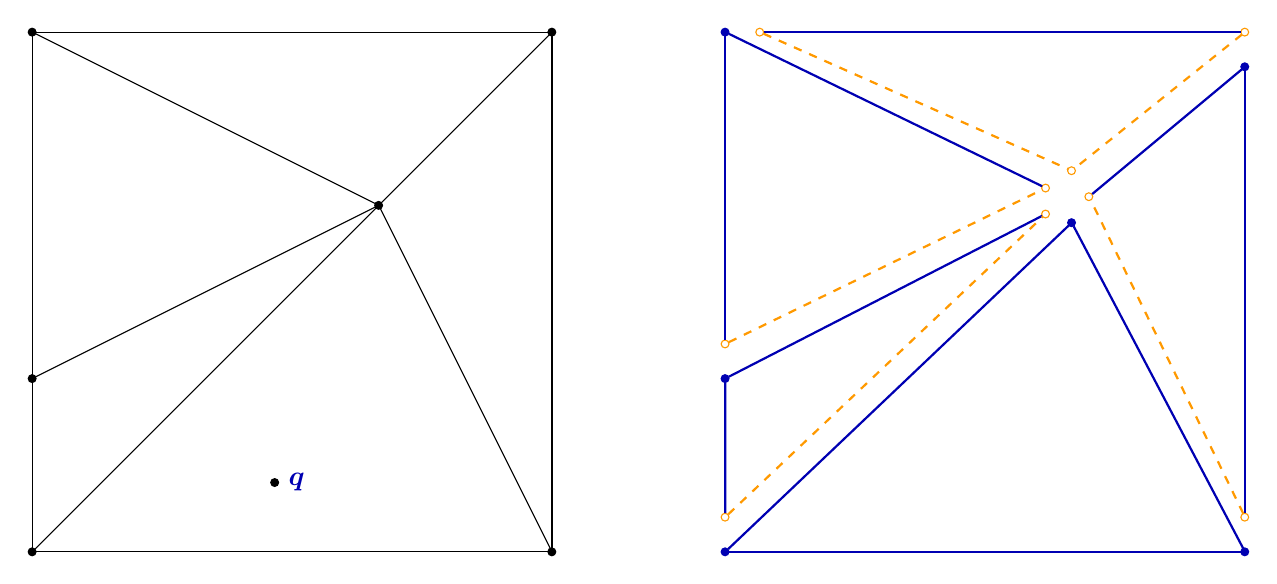
\begin{tikzpicture}[scale=2.2]
                \node[fill=black, draw=black, shape=circle, scale=0.3] (a) at (4,3) {} ;
                \node[fill=black, draw=black, shape=circle, scale=0.3](ab) at (4,1) {} ;
                \node[fill=black, draw=black, shape=circle, scale=0.3](b) at (4,0) {} ;
                \node[fill=black, draw=black, shape=circle, scale=0.3](c) at (7,3) {} ;
                \node[fill=black, draw=black, shape=circle, scale=0.3](d) at (7,0) {} ;
                \node[fill=black, draw=black, shape=circle, scale=0.3](x) at (6,2) {} ;
                \node[fill=black, draw=black, shape=circle, scale=0.3,
label={right:\bm \q \em}](q) at (5.4, 0.4) {} ;
                \draw (a) -- (b) ;
                \draw (c) -- (d) ;
                \draw (a) -- (c) ;
                \draw (b) -- (d) ;
                \draw (a) -- (x) ;
                \draw (b) -- (x) ;
                \draw (c) -- (x) ;
                \draw (d) -- (x) ;
                \draw (ab) -- (x) ;

                
                \node[fill=blue, draw=blue, shape=circle, scale=0.3] (a-closed) at (8,3) {} ;
                \node[fill=none, draw=orange, shape=circle, scale=0.3] (a-open) at (8.2,3) {} ;
                \node[fill=none, draw=orange, shape=circle, scale=0.3](ab-open) at (8,1.2) {} ;
                \node[fill=blue, draw=blue, shape=circle, scale=0.3](ab-closed) at (8,1) {} ;
                \node[fill=blue, draw=blue, shape=circle, scale=0.3](b-closed) at (8,0) {} ;
                \node[fill=none, draw=orange, shape=circle, scale=0.3](b-open) at (8,0.2) {} ;
                \node[fill=none, draw=orange, shape=circle, scale=0.3](c-open) at (11,3) {} ;
                \node[fill=blue, draw=blue, shape=circle, scale=0.3](c-closed) at (11,2.8) {} ;
                \node[fill=none, draw=orange, shape=circle, scale=0.3](d-open) at (11,0.2) {} ;
                \node[fill=blue, draw=blue, shape=circle, scale=0.3](d-closed) at (11,0) {} ;
                \node[fill=blue, draw=blue, shape=circle, scale=0.3](x-b-d) at (10,1.9) {} ;
                \node[fill=none, draw=orange, shape=circle, scale=0.3](x-b-ab) at (9.85,1.95) {} ;
                \node[fill=none, draw=orange, shape=circle, scale=0.3](x-ab-a) at (9.85,2.1) {} ;
                \node[fill=none, draw=orange, shape=circle, scale=0.3](x-a-c) at (10,2.2) {} ;
                \node[fill=none, draw=orange, shape=circle, scale=0.3](x-c-d) at (10.1,2.05) {} ;
                \draw[thick,blue] (b-open) -- (ab-closed) ;
                \draw[thick,blue] (ab-open) -- (a-closed) ;
                \draw[thick, blue] (a-open) -- (c-open) ;
                \draw[thick, blue] (c-closed) -- (d-open) ;
                \draw[thick, blue] (d-closed) -- (b-closed) ;
                \draw[thick, blue] (b-closed) -- (x-b-d) ;
                \draw[thick, blue] (d-closed) -- (x-b-d) ;
                \draw[thick, orange, dashed] (d-open) -- (x-c-d) ;
                \draw[thick, blue] (c-closed) -- (x-c-d) ;
                \draw[thick, orange, dashed] (c-open) -- (x-a-c) ;
                \draw[thick, orange, dashed] (a-open) -- (x-a-c) ;
                \draw[thick, blue] (a-closed) -- (x-ab-a) ;
                \draw[thick, orange, dashed] (ab-open) -- (x-ab-a) ;
                \draw[thick, blue] (ab-closed) -- (x-b-ab) ;
                \draw[thick, orange, dashed] (b-open) -- (x-b-ab) ;

\end{tikzpicture}

\thawpage
\freezepage
%%%%%%%%%%%%%%%%%%%%%%%%%%%%%%%%%%%%%%%%%%%%%%%%%%%%%

\foilhead[-20pt]{\green Tangent Cones \& Visibility}

\bm \F \em facet of a polyhedron \bm \P \subset \R^d \em with defining halfspace \bm H \em

\bm \F \em is \red visible \black from \bm \q \in \R^d \em if \bm \q \notin H \em

%\vspace{-.1in}
\hspace{1.4in}
\includegraphics[totalheight=3in]{../../../CRT-Book/David/beneath-beyond-cone}

Equivalent lingo: \bm \q \in \R^d \em is \red beyond \bm \F \em (and \red beneath
\black otherwise)

%%%%%%%%%%%%%%%%%%%%%%%%%%%%%%%%%%%%%%%%%%%%%%%%%%%%%

\foilhead[-20pt]{\green Half-open Triangulations}

Define \bm \hopen_\q (\cQ) \em to be \bm \cQ \em minus facets that are visible from \bm \q \em

\red Exercise
\bm \P \subset \R^d \em --- full-dimensional polyhedron with dissection \bm \P = \P_1
\cup \P_2 \cup \cdots \cup \P_m \em\!\!, 
\bm \q \in \R^d \em generic relative to each \bm \P_j \em
\green \quad $\longrightarrow$
\be
  \hopen_\q \P \ = \ \hopen_\q \P_1 \uplus \hopen_\q \P_2 \uplus \cdots \uplus \hopen_\q \P_m
\ee

\vspace{-.3in}
\hspace{1.3in}
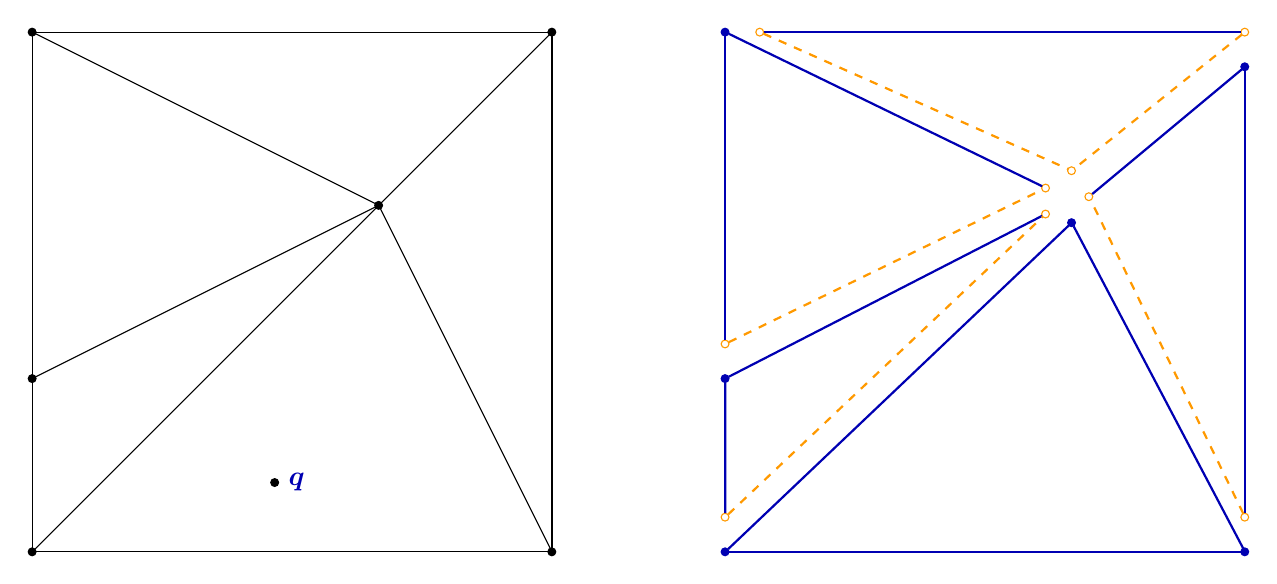
\begin{tikzpicture}[scale=2.2]
                \node[fill=black, draw=black, shape=circle, scale=0.3] (a) at (4,3) {} ;
                \node[fill=black, draw=black, shape=circle, scale=0.3](ab) at (4,1) {} ;
                \node[fill=black, draw=black, shape=circle, scale=0.3](b) at (4,0) {} ;
                \node[fill=black, draw=black, shape=circle, scale=0.3](c) at (7,3) {} ;
                \node[fill=black, draw=black, shape=circle, scale=0.3](d) at (7,0) {} ;
                \node[fill=black, draw=black, shape=circle, scale=0.3](x) at (6,2) {} ;
                \node[fill=black, draw=black, shape=circle, scale=0.3,
label={right:\bm \q \em}](q) at (5.4, 0.4) {} ;
                \draw (a) -- (b) ;
                \draw (c) -- (d) ;
                \draw (a) -- (c) ;
                \draw (b) -- (d) ;
                \draw (a) -- (x) ;
                \draw (b) -- (x) ;
                \draw (c) -- (x) ;
                \draw (d) -- (x) ;
                \draw (ab) -- (x) ;

                
                \node[fill=blue, draw=blue, shape=circle, scale=0.3] (a-closed) at (8,3) {} ;
                \node[fill=none, draw=orange, shape=circle, scale=0.3] (a-open) at (8.2,3) {} ;
                \node[fill=none, draw=orange, shape=circle, scale=0.3](ab-open) at (8,1.2) {} ;
                \node[fill=blue, draw=blue, shape=circle, scale=0.3](ab-closed) at (8,1) {} ;
                \node[fill=blue, draw=blue, shape=circle, scale=0.3](b-closed) at (8,0) {} ;
                \node[fill=none, draw=orange, shape=circle, scale=0.3](b-open) at (8,0.2) {} ;
                \node[fill=none, draw=orange, shape=circle, scale=0.3](c-open) at (11,3) {} ;
                \node[fill=blue, draw=blue, shape=circle, scale=0.3](c-closed) at (11,2.8) {} ;
                \node[fill=none, draw=orange, shape=circle, scale=0.3](d-open) at (11,0.2) {} ;
                \node[fill=blue, draw=blue, shape=circle, scale=0.3](d-closed) at (11,0) {} ;
                \node[fill=blue, draw=blue, shape=circle, scale=0.3](x-b-d) at (10,1.9) {} ;
                \node[fill=none, draw=orange, shape=circle, scale=0.3](x-b-ab) at (9.85,1.95) {} ;
                \node[fill=none, draw=orange, shape=circle, scale=0.3](x-ab-a) at (9.85,2.1) {} ;
                \node[fill=none, draw=orange, shape=circle, scale=0.3](x-a-c) at (10,2.2) {} ;
                \node[fill=none, draw=orange, shape=circle, scale=0.3](x-c-d) at (10.1,2.05) {} ;
                \draw[thick,blue] (b-open) -- (ab-closed) ;
                \draw[thick,blue] (ab-open) -- (a-closed) ;
                \draw[thick, blue] (a-open) -- (c-open) ;
                \draw[thick, blue] (c-closed) -- (d-open) ;
                \draw[thick, blue] (d-closed) -- (b-closed) ;
                \draw[thick, blue] (b-closed) -- (x-b-d) ;
                \draw[thick, blue] (d-closed) -- (x-b-d) ;
                \draw[thick, orange, dashed] (d-open) -- (x-c-d) ;
                \draw[thick, blue] (c-closed) -- (x-c-d) ;
                \draw[thick, orange, dashed] (c-open) -- (x-a-c) ;
                \draw[thick, orange, dashed] (a-open) -- (x-a-c) ;
                \draw[thick, blue] (a-closed) -- (x-ab-a) ;
                \draw[thick, orange, dashed] (ab-open) -- (x-ab-a) ;
                \draw[thick, blue] (ab-closed) -- (x-b-ab) ;
                \draw[thick, orange, dashed] (b-open) -- (x-b-ab) ;

\end{tikzpicture}

%%%%%%%%%%%%%%%%%%%%%%%%%%%%%%%%%%%%%%%%%%%%%%%%%%%%%

\foilhead[-20pt]{\green Recall: Integer-point Complexity of a Simplicial Cone}

What if \bm \K \em is (still simplicial and rational but) not unimodular?
\\
Say \bm \w_1, \w_2, \w_3 \in \Z^3 \em are linearly independent,
\bm \det [\w_1 \, \w_2 \, \w_3] = D > 1 \em

\bm \K = \R_{ \ge 0 } \, \w_1 + \R_{ \ge 0 } \, \w_2 + \R_{ \ge 0 } \, \w_3 \em

\red Idea \black \ Tile \bm \K \em with the half-open parallelepiped
\\
\bm \Pi = [0,1) \, \w_1 + [0,1) \, \w_2 + [0,1) \, \w_3 \em

\vspace{-1.9in}
\hspace{5.8in}
\includegraphics[totalheight=3in]{../../../CRT-Book/David/3dim-tiling-domain}

\vspace{-1.4in}
\includegraphics[totalheight=3in]{../../../CRT-Book/David/3dim-tiling}

\vspace{-3.5in}
\hspace{4.2in}
\green $\downarrow$

\hspace{3.7in}
\bm \sigma_\K(z_1, z_2, z_3) = \em

\vspace{-.2in}
\hspace{3.7in}
\bm \displaystyle \frac{ \sigma_\Pi(z_1, z_2, z_3) }{ (1 - \z^{ \w_1 }) (1 - \z^{
\w_2 }) (1 - \z^{ \w_3 })  } \em

\hspace{3.7in}
where \bm \z^\m = z_1^{ m_1 } z_2^{ m_2 } z_3^{ m_3 } \em

\thawpage
\freezepage
%%%%%%%%%%%%%%%%%%%%%%%%%%%%%%%%%%%%%%%%%%%%%%%%%%%%%

\foilhead[-20pt]{\green Recall: Homogenizing Polytopes}

Given a polytope \bm \P \subset \R^d \em let

\bm \cone(\P) \, := \, \R_{ \ge 0 } \left( \P \times \{ 1 \} \right) \subset \R^{
d+1 } \em

\vspace{-.2in}
\bm = \, \R_{ \ge 0 } \begin{bmatrix} \v_1 \\ 1 \end{bmatrix} 
  + \R_{ \ge 0 } \begin{bmatrix} \v_2 \\ 1 \end{bmatrix}
  + \dots + \R_{ \ge 0 } \begin{bmatrix} \v_n \\ 1 \end{bmatrix} \em

\vspace{-2.9in}
\hspace{5.2in}
\includegraphics[totalheight=4in]{../../David/titlepicturenolables-eps-converted-to}

\vspace{-1.1in}
\bm \cone(\P) \cap \{ \x \in \R^{ d+1 } : \, x_{ d+1 } = t \} \em
% = t\P \times \{ t \} \em

\vspace{-.2in}
contains a copy of \bm t\P \em \ \green $\longrightarrow$

\vspace{-.4in}
\be \displaystyle \Ehr_\P (z) \, := \, 1 + \sum_{ t \ge 1 } L_\P (t) \, z^t 
\, = \, \sigma_{ \cone(\P) } (1, 1, \dots, 1, z) \ee

\vspace{-.5in}
If \bm \P \em is a simplex,

\vspace{-.3in}
\hspace{.6in}
\bm \displaystyle \sigma_{ \cone(\P) } (\z) \, = \, \frac{ \sigma_\Pi(\z) }{ \displaystyle \prod_{
\v \text{ vertex } } (1 - \z^\v ) } \em
\ \ \ \green $\longrightarrow$ \ \ \ 
\bm \displaystyle  \Ehr_\P (z) \, = \, \frac{ h^*_\P(z) }{ (1-z)^{ d+1 } } \em

%%%%%%%%%%%%%%%%%%%%%%%%%%%%%%%%%%%%%%%%%%%%%%%%%%%%%

\foilhead[-29pt]{\green Ehrhart Positivity}

\hspace{1.8in}
\red Theorem \black
(Ehrhart 1962) 
For any lattice polytope \bm \P \em\!\!,

\vspace{-.4in}
\hspace{1.8in}
\bm L_\P (t) \em is a polynomial in \bm t \em of
degree \bm d := \dim \P \em with 

\vspace{-.4in}
\hspace{1.8in}
leading coefficient \bm \vol \P \em %(normalized to \bm \aff \P \cap \Z^d \em\!\!) 
and constant term \bm 1 \em\!\!.

\vspace{-.1in}
\hspace{2.2in}
\bm \displaystyle \Ehr_\P (z) \, := \, 1 + \sum_{ t \ge 1 } L_\P (t) \, z^t \, = \,
\dfrac{ h_\P^*(z) }{ (1-z)^{ d + 1 } } \em

\vspace{-2.9in}
\includegraphics[totalheight=2.5in]{../ehrhart}

\red Theorem \black (Stanley 1980) \bm h^*_0, h^*_1, \dots, h^*_d \em are nonnegative integers.

%%%%%%%%%%%%%%%%%%%%%%%%%%%%%%%%%%%%%%%%%%%%%%%%%%%%%

\foilhead[-29pt]{\green Ehrhart Positivity}

\hspace{1.8in}
\red Theorem \black
(Ehrhart 1962) 
For any lattice polytope \bm \P \em\!\!,

\vspace{-.4in}
\hspace{1.8in}
\bm L_\P (t) \em is a polynomial in \bm t \em of
degree \bm d := \dim \P \em with 

\vspace{-.4in}
\hspace{1.8in}
leading coefficient \bm \vol \P \em %(normalized to \bm \aff \P \cap \Z^d \em\!\!) 
and constant term \bm 1 \em\!\!.

\vspace{-.1in}
\hspace{2.2in}
\bm \displaystyle \Ehr_\P (z) \, := \, 1 + \sum_{ t \ge 1 } L_\P (t) \, z^t \, = \,
\dfrac{ h_\P^*(z) }{ (1-z)^{ d + 1 } } \em

\vspace{-2.9in}
\includegraphics[totalheight=2.5in]{../ehrhart}

\red Theorem \black (Stanley 1980) \bm h^*_0, h^*_1, \dots, h^*_d \em are nonnegative integers.

\red Open Problem \black \ Prove that the \bm h^* \em\!\!-polynomial of \\
\mybullet hypersimplices \\
\mybullet polytopes admitting a unimodular triangulation \\
\mybullet polytope with the integer decomposition property 
are \red unimodal

\green $\checkmark$ \black Gorenstein polytopes with regular
unimodular triangulation (Bruns-- \\
\mbox{} \ \ \  R\"omer 2007) \\
\green $\checkmark$ \black Zonotopes (\MB\!--Jochemko--McCullough 2019)

%%%%%%%%%%%%%%%%%%%%%%%%%%%%%%%%%%%%%%%%%%%%%%%%%%%%%

\foilhead[-20pt]{\green Recall:$^2$ Integer-point Complexity of a Simplicial Cone}

What if \bm \K \em is (still simplicial and rational but) not unimodular?
\\
Say \bm \w_1, \w_2, \w_3 \in \Z^3 \em are linearly independent,
\bm \det [\w_1 \, \w_2 \, \w_3] = D > 1 \em

\bm \K = \R_{ \ge 0 } \, \w_1 + \R_{ \ge 0 } \, \w_2 + \R_{ \ge 0 } \, \w_3 \em

\red Idea \black \ Tile \bm \K \em with the half-open parallelepiped
\\
\bm \Pi = [0,1) \, \w_1 + [0,1) \, \w_2 + [0,1) \, \w_3 \em

\vspace{-1.9in}
\hspace{5.8in}
\includegraphics[totalheight=3in]{../../../CRT-Book/David/3dim-tiling-domain}

\vspace{-1.4in}
\includegraphics[totalheight=3in]{../../../CRT-Book/David/3dim-tiling}

\vspace{-3.5in}
\hspace{4.2in}
\green $\downarrow$

\hspace{3.7in}
\bm \sigma_\K(z_1, z_2, z_3) = \em

\vspace{-.2in}
\hspace{3.7in}
\bm \displaystyle \frac{ \sigma_\Pi(z_1, z_2, z_3) }{ (1 - \z^{ \w_1 }) (1 - \z^{
\w_2 }) (1 - \z^{ \w_3 })  } \em

\hspace{3.7in}
where \bm \z^\m = z_1^{ m_1 } z_2^{ m_2 } z_3^{ m_3 } \em

\thawpage
\freezepage
%%%%%%%%%%%%%%%%%%%%%%%%%%%%%%%%%%%%%%%%%%%%%%%%%%%%%

\foilhead[-20pt]{\green Simplicial Cone Reciprocity}

\bm \v_1, \v_2, \dots, \v_k \in \Z^d \em linearly independent
%
\ba
        \Chat &:=& \R_{ \ge 0 } \v_1 + \dots + \R_{ \ge 0 } \v_{ m-1 } +
        \R_{ >0 } \v_m + \dots + \R_{ >0 } \v_k \\
        \Ccheck &:=& \R_{ >0 } \v_1 + \dots + \R_{ >0 } \v_{ m-1 } + \R_{
        \ge 0 } \v_m + \dots + \R_{ \ge 0 } \v_k 
\ea
 \ \ \quad \quad \quad \green $\downarrow$
\be
  \sigma_{ \Chat } (\z)
  \, = \, \frac{ \sigma_{ \PPhat } (\z) }{ \left( 1 - \z^{ \v_1 } \right) \cdots \left( 1 - \z^{ \v_k } \right) }
\qquad \qquad
  \sigma_{ \Ccheck } (\z)
  \, = \, \frac{ \sigma_{ \PPcheck } (\z) }{ \left( 1 - \z^{ \v_1 } \right) \cdots \left( 1 - \z^{ \v_k } \right) }
\ee
where
\ba
\PPhat &:=& [0,1) \, \v_1 + \dots + [0,1) \, \v_{ m-1 } + (0,1] \, \v_m + \dots +
(0,1] \, \v_k \\
\PPcheck &:=& (0,1] \, \v_1 + \dots + (0,1] \, \v_{ m-1 } + [0,1) \, \v_m + \dots + [0,1) \, \v_k 
\ea

%%%%%%%%%%%%%%%%%%%%%%%%%%%%%%%%%%%%%%%%%%%%%%%%%%%%%

\foilhead[-20pt]{\green Simplicial Cone Reciprocity}

\bm \v_1, \v_2, \dots, \v_k \in \Z^d \em linearly independent
%
\ba
\PPhat &:=& [0,1) \, \v_1 + \dots + [0,1) \, \v_{ m-1 } + (0,1] \, \v_m + \dots +
(0,1] \, \v_k \\
\PPcheck &:=& (0,1] \, \v_1 + \dots + (0,1] \, \v_{ m-1 } + [0,1) \, \v_m + \dots + [0,1) \, \v_k 
\ea
%
\red Fun Fact \ \ \bm \PPhat \, = \, \v_1 + \v_2 + \dots + \v_k -  \PPcheck \em

\vspace{-.2in}
\hspace{.4in}
\includegraphics[totalheight=2.6in]{../../../CRT-Book/David/two-parallelpipeds}

%%%%%%%%%%%%%%%%%%%%%%%%%%%%%%%%%%%%%%%%%%%%%%%%%%%%%

\foilhead[-20pt]{\green Simplicial Cone Reciprocity}

\bm \v_1, \v_2, \dots, \v_k \in \Z^d \em linearly independent
%
\ba
\PPhat &:=& [0,1) \, \v_1 + \dots + [0,1) \, \v_{ m-1 } + (0,1] \, \v_m + \dots +
(0,1] \, \v_k \\
\PPcheck &:=& (0,1] \, \v_1 + \dots + (0,1] \, \v_{ m-1 } + [0,1) \, \v_m + \dots + [0,1) \, \v_k 
\ea
%
\red Fun Fact \ \ \bm \PPhat \, = \, \v_1 + \v_2 + \dots + \v_k -  \PPcheck \em

\vspace{-.2in}
\hspace{.4in}
\includegraphics[totalheight=2.6in]{../../../CRT-Book/David/two-parallelpipeds}

\green $\longrightarrow$ \ 
\bm \displaystyle \sigma_{ \PPhat } (\z) \, = \, \z^{ \v_1 + \v_2 + \dots + \v_k }\,\sigma_{ \PPcheck }\left( \frac 1 \z \right) \em

%%%%%%%%%%%%%%%%%%%%%%%%%%%%%%%%%%%%%%%%%%%%%%%%%%%%%

\foilhead[-20pt]{\green Stanley Reciprocity}

\vspace{-.6in}
\be
  \sigma_{ \Chat } (\z)
  \, = \, \frac{ \sigma_{ \PPhat } (\z) }{ \left( 1 - \z^{ \v_1 } \right) \cdots \left( 1 - \z^{ \v_k } \right) }
\qquad \qquad
  \sigma_{ \Ccheck } (\z)
  \, = \, \frac{ \sigma_{ \PPcheck } (\z) }{ \left( 1 - \z^{ \v_1 } \right) \cdots \left( 1 - \z^{ \v_k } \right) }
\ee

\vspace{-.4in}
\bm \displaystyle \ \ \sigma_{ \PPhat } (\z) \, = \, \z^{ \v_1 + \v_2 + \dots + \v_k }\,\sigma_{ \PPcheck }\left( \frac 1 \z \right) \em
\qquad \quad \green $\longrightarrow$ \ 
\ba
  \sigma_{ \Ccheck } \left( \frac 1 \z \right)
  &=& \frac{ \sigma_{ \PPcheck } (\frac 1 \z) }{ \left( 1 - \z^{ -\v_1 } \right) \cdots \left( 1 - \z^{ -\v_k } \right) }
  \ = \ \frac{\z^{ -\v_1 - \v_2 - \dots - \v_k } \, \sigma_{ \PPhat } (\z)  }{ \left( 1 - \z^{ -\v_1 } \right) \cdots \left( 1 - \z^{ -\v_k } \right) } \\ &=& (-1)^k \frac{ \sigma_{ \PPhat } (\z) }{ \left( 1 - \z^{ \v_1 } \right) \cdots \left( 1 - \z^{ \v_
k } \right) }
  \ = \ (-1)^k \, \sigma_{ \Chat } (\z) 
\ea

\thawpage
\freezepage
%%%%%%%%%%%%%%%%%%%%%%%%%%%%%%%%%%%%%%%%%%%%%%%%%%%%%%

\foilhead[-20pt]{\green Stanley Reciprocity}

\vspace{-.6in}
\be
  \sigma_{ \Chat } (\z)
  \, = \, \frac{ \sigma_{ \PPhat } (\z) }{ \left( 1 - \z^{ \v_1 } \right) \cdots \left( 1 - \z^{ \v_k } \right) }
\qquad \qquad
  \sigma_{ \Ccheck } (\z)
  \, = \, \frac{ \sigma_{ \PPcheck } (\z) }{ \left( 1 - \z^{ \v_1 } \right) \cdots \left( 1 - \z^{ \v_k } \right) }
\ee

\vspace{-.4in}
\bm \displaystyle \ \ \sigma_{ \PPhat } (\z) \, = \, \z^{ \v_1 + \v_2 + \dots + \v_k }\,\sigma_{ \PPcheck }\left( \frac 1 \z \right) \em
\qquad \quad \green $\longrightarrow$ \ 
\ba
  \sigma_{ \Ccheck } \left( \frac 1 \z \right)
  &=& \frac{ \sigma_{ \PPcheck } (\frac 1 \z) }{ \left( 1 - \z^{ -\v_1 } \right) \cdots \left( 1 - \z^{ -\v_k } \right) }
  \ = \ \frac{\z^{ -\v_1 - \v_2 - \dots - \v_k } \, \sigma_{ \PPhat } (\z)  }{ \left( 1 - \z^{ -\v_1 } \right) \cdots \left( 1 - \z^{ -\v_k } \right) } \\ &=& (-1)^k \frac{ \sigma_{ \PPhat } (\z) }{ \left( 1 - \z^{ \v_1 } \right) \cdots \left( 1 - \z^{ \v_
k } \right) }
  \ = \ (-1)^k \, \sigma_{ \Chat } (\z) 
\ea
%
\red Theorem \black (Stanley) \
Let \bm \K \subset \R^d \em be a full-dimensional pointed rational cone, and let \bm
\q \in \R^d \em be generic relative to \bm \K \em\!\!.
Then

\vspace{-.5in}
\hspace{5.1in}
\bm \displaystyle
  \sigma_{ \hopen_\q \K } \left( \frac 1 \z \right) \, = \, (-1)^d \, \sigma_{ \hopen^\q \K } (\z) 
\em

%%%%%%%%%%%%%%%%%%%%%%%%%%%%%%%%%%%%%%%%%%%%%%%%%%%%%%

\foilhead[-20pt]{\green Stanley Reciprocity}

\vspace{-.6in}
\be
  \sigma_{ \Chat } (\z)
  \, = \, \frac{ \sigma_{ \PPhat } (\z) }{ \left( 1 - \z^{ \v_1 } \right) \cdots \left( 1 - \z^{ \v_k } \right) }
\qquad \qquad
  \sigma_{ \Ccheck } (\z)
  \, = \, \frac{ \sigma_{ \PPcheck } (\z) }{ \left( 1 - \z^{ \v_1 } \right) \cdots \left( 1 - \z^{ \v_k } \right) }
\ee

\vspace{-.4in}
\bm \displaystyle \ \ \sigma_{ \PPhat } (\z) \, = \, \z^{ \v_1 + \v_2 + \dots + \v_k }\,\sigma_{ \PPcheck }\left( \frac 1 \z \right) \em
\qquad \quad \green $\longrightarrow$ \ 
\ba
  \sigma_{ \Ccheck } \left( \frac 1 \z \right)
  &=& \frac{ \sigma_{ \PPcheck } (\frac 1 \z) }{ \left( 1 - \z^{ -\v_1 } \right) \cdots \left( 1 - \z^{ -\v_k } \right) }
  \ = \ \frac{\z^{ -\v_1 - \v_2 - \dots - \v_k } \, \sigma_{ \PPhat } (\z)  }{ \left( 1 - \z^{ -\v_1 } \right) \cdots \left( 1 - \z^{ -\v_k } \right) } \\ &=& (-1)^k \frac{ \sigma_{ \PPhat } (\z) }{ \left( 1 - \z^{ \v_1 } \right) \cdots \left( 1 - \z^{ \v_
k } \right) }
  \ = \ (-1)^k \, \sigma_{ \Chat } (\z) 
\ea
%
\red Theorem \black (Stanley) \
Let \bm \K \subset \R^d \em be a full-dimensional pointed rational cone, and let \bm
\q \in \R^d \em be generic relative to \bm \K \em\!\!.
Then

\vspace{-.5in}
\hspace{5.1in}
\bm \displaystyle
  \sigma_{ \hopen_\q \K } \left( \frac 1 \z \right) \, = \, (-1)^d \, \sigma_{ \hopen^\q \K } (\z) 
\em

\vspace{-.4in}
\red Corollary \black \
\bm \displaystyle \sigma_{ \K } \left( \frac 1 \z \right) \, = \, (-1)^d \, \sigma_{
\K^\circ } (\z) \em

%%%%%%%%%%%%%%%%%%%%%%%%%%%%%%%%%%%%%%%%%%%%%%%%%%%%%

\foilhead[-20pt]{\green Ehrhart--Macdonald Reciprocity}

\red Corollary \black (Stanley) \
Let \bm \K \subset \R^d \em be a full-dimensional pointed rational cone, and let \bm
\q \in \R^d \em be generic relative to \bm \K \em\!\!.
Then

\vspace{-.5in}
\hspace{5.5in}
\bm \displaystyle \sigma_{ \K } \left( \frac 1 \z \right) \, = \, (-1)^d \, \sigma_{
\K^\circ } (\z) \em

\vspace{-.4in}
\ba 
  \Ehr_\P (z)
  &\!\!\!:=& \!\!\!1 + \sum_{ t \ge 1 } L_\P (t) \, z^t
  \, = \, \dfrac{ h_\P^*(z) }{ (1-z)^{ d + 1 } } 
  \, = \, \sigma_{ \cone(\P) } (1, 1, \dots, z) \\
  \Ehr_{\P^\circ} (z)
  &\!\!\!:=& \!\!\!\sum_{ t \ge 1 } L_{\P^\circ} (t) \, z^t
  \, = \, \sigma_{ \cone(\P)^\circ } (1, 1, \dots, z) 
\ea

\thawpage
\freezepage
%%%%%%%%%%%%%%%%%%%%%%%%%%%%%%%%%%%%%%%%%%%%%%%%%%%%%%

\foilhead[-20pt]{\green Ehrhart--Macdonald Reciprocity}

\red Corollary \black (Stanley) \
Let \bm \K \subset \R^d \em be a full-dimensional pointed rational cone, and let \bm
\q \in \R^d \em be generic relative to \bm \K \em\!\!.
Then

\vspace{-.5in}
\hspace{5.5in}
\bm \displaystyle \sigma_{ \K } \left( \frac 1 \z \right) \, = \, (-1)^d \, \sigma_{
\K^\circ } (\z) \em

\vspace{-.4in}
\ba 
  \Ehr_\P (z)
  &\!\!\!:=& \!\!\!1 + \sum_{ t \ge 1 } L_\P (t) \, z^t
  \, = \, \dfrac{ h_\P^*(z) }{ (1-z)^{ d + 1 } } 
  \, = \, \sigma_{ \cone(\P) } (1, 1, \dots, z) \\
  \Ehr_{\P^\circ} (z)
  &\!\!\!:=& \!\!\!\sum_{ t \ge 1 } L_{\P^\circ} (t) \, z^t
  \, = \, \sigma_{ \cone(\P)^\circ } (1, 1, \dots, z) 
\ea
%
\red Corollary$^2$ \black  \
Let \bm \P \em be a lattice \bm d \em\!\!-polytope. Then
\be
  \Ehr_{\P^\circ} (z) \, = \, \dfrac{ z^{ d+1 } \, h_\P^*(\frac 1 z) }{ (1-z)^{ d + 1 } } 
  \, = \, (-1)^{d+1} \, \Ehr_\P \left( \frac 1 z \right)
\ee 

%%%%%%%%%%%%%%%%%%%%%%%%%%%%%%%%%%%%%%%%%%%%%%%%%%%%%%%

\foilhead[-20pt]{\green Ehrhart--Macdonald Reciprocity}

\red Corollary \black (Stanley) \
Let \bm \K \subset \R^d \em be a full-dimensional pointed rational cone, and let \bm
\q \in \R^d \em be generic relative to \bm \K \em\!\!.
Then

\vspace{-.5in}
\hspace{5.5in}
\bm \displaystyle \sigma_{ \K } \left( \frac 1 \z \right) \, = \, (-1)^d \, \sigma_{
\K^\circ } (\z) \em

\vspace{-.4in}
\ba 
  \Ehr_\P (z)
  &\!\!\!:=& \!\!\!1 + \sum_{ t \ge 1 } L_\P (t) \, z^t
  \, = \, \dfrac{ h_\P^*(z) }{ (1-z)^{ d + 1 } } 
  \, = \, \sigma_{ \cone(\P) } (1, 1, \dots, z) \\
  \Ehr_{\P^\circ} (z)
  &\!\!\!:=& \!\!\!\sum_{ t \ge 1 } L_{\P^\circ} (t) \, z^t
  \, = \, \sigma_{ \cone(\P)^\circ } (1, 1, \dots, z) 
\ea
%
\red Corollary$^2$ \black  \
Let \bm \P \em be a lattice \bm d \em\!\!-polytope. Then
\be
  \Ehr_{\P^\circ} (z) \, = \, \dfrac{ z^{ d+1 } \, h_\P^*(\frac 1 z) }{ (1-z)^{ d + 1 } } 
  \, = \, (-1)^{d+1} \, \Ehr_\P \left( \frac 1 z \right)
\ee 
%
\red Corollary$^3$ \black (Ehrhart--Macdonald) \ \ 
\bm \displaystyle L_\P \left( \frac 1 t \right) \, = \, (-1)^{d} \, L_{\P^\circ} (t) \em 

%%%%%%%%%%%%%%%%%%%%%%%%%%%%%%%%%%%%%%%%%%%%%%%%%%%%%

\foilhead[-29pt]{\green Order Polytopes}

\bm (\Pi,\preceq) \em --- finite partially ordered set (\red poset \black\!\!)
%
\be
    \OP_\Pi \ := \ \left\{ \phi \in \R^\Pi :
    \begin{array}{cl}
        0        \le \phi(p) \le 1 & \text{for all } p \in \Pi \\
        \phi(a)  \le \phi(b) & \text{whenever } a \preceq b
    \end{array}
    \right\}
\ee

\thawpage
\freezepage
%%%%%%%%%%%%%%%%%%%%%%%%%%%%%%%%%%%%%%%%%%%%%%%%%%%%%

\foilhead[-29pt]{\green Order Polytopes}

\bm (\Pi,\preceq) \em --- finite partially ordered set (\red poset \black\!\!)
%
\be
    \OP_\Pi \ := \ \left\{ \phi \in \R^\Pi :
    \begin{array}{cl}
        0        \le \phi(p) \le 1 & \text{for all } p \in \Pi \\
        \phi(a)  \le \phi(b) & \text{whenever } a \preceq b
    \end{array}
    \right\}
\ee
%
Integer points in \bm t \, \OP_\Pi \em correspond to \red
order preserving maps \bm \Pi \to \{ 0, 1, \dots, t \} \em

%%%%%%%%%%%%%%%%%%%%%%%%%%%%%%%%%%%%%%%%%%%%%%%%%%%%%

\foilhead[-29pt]{\green Order Polytopes}

\bm (\Pi,\preceq) \em --- finite partially ordered set (\red poset \black\!\!)
%
\be
    \OP_\Pi \ := \ \left\{ \phi \in \R^\Pi :
    \begin{array}{cl}
        0        \le \phi(p) \le 1 & \text{for all } p \in \Pi \\
        \phi(a)  \le \phi(b) & \text{whenever } a \preceq b
    \end{array}
    \right\}
\ee
%
Integer points in \bm t \, \OP_\Pi \em correspond to \red
order preserving maps \bm \Pi \to \{ 0, 1, \dots, t \} \em

\vspace{-.4in}
those in \bm t \, \OP_\Pi^\circ \em correspond to \red
strictly order preserving maps \bm \Pi \to \{ 1, \dots, t-1 \} \em
\be
  \phi(a) < \phi(b) \qquad  \text{whenever } a \prec b
\ee

\vspace{-.4in}
Ehrhart--Macdonald Reciprocity
\ \green $\longrightarrow$ \
\bm \displaystyle L_{\OP_\Pi} \left( \frac 1 t \right) \, = \, (-1)^{|\Pi|} \, L_{\OP_\Pi^\circ} (t) \em 

%%%%%%%%%%%%%%%%%%%%%%%%%%%%%%%%%%%%%%%%%%%%%%%%%%%%%

\foilhead[-20pt]{\headercolor Back to Graph Colorings}

\bm \Gamma = (V,E) \em --- graph (without loops)

\red Proper \bm n \em\!\!\red-coloring \black of \bm \Gamma \em --- \bm \x \in \{ 1, 2, \dots, n \}^V \em such that \bm x_i \not= x_j \em if \bm ij \in E \em

An orientation \bm \alpha \em of \bm \Gamma \em is \red acyclic \black if it has no directed cycles
\ \green $\longrightarrow$ \ \black
poset \bm \Pi_\alpha \em

\thawpage
\freezepage
%%%%%%%%%%%%%%%%%%%%%%%%%%%%%%%%%%%%%%%%%%%%%%%%%%%%%

\foilhead[-20pt]{\headercolor Back to Graph Colorings}

\bm \Gamma = (V,E) \em --- graph (without loops)

\red Proper \bm n \em\!\!\red-coloring \black of \bm \Gamma \em --- \bm \x \in \{ 1, 2, \dots, n \}^V \em such that \bm x_i \not= x_j \em if \bm ij \in E \em

An orientation \bm \alpha \em of \bm \Gamma \em is \red acyclic \black if it has no directed cycles
\ \green $\longrightarrow$ \ \black
poset \bm \Pi_\alpha \em

Graph Coloring a la Ehrhart: \

\bm \displaystyle \chi_\Gamma (n) \, = \, \sum_{ \alpha } L_{\OP_{\Pi_\alpha}^\circ} (n+1) \em

\vspace{-1.3in}
\hspace{3.4in}
\includegraphics[totalheight=3.5in]{../../../CRT-Book/David/order-polynomial}

%%%%%%%%%%%%%%%%%%%%%%%%%%%%%%%%%%%%%%%%%%%%%%%%%%%%%

\foilhead[-20pt]{\headercolor Back to Graph Colorings}

\bm \Gamma = (V,E) \em --- graph (without loops)

\red Proper \bm n \em\!\!\red-coloring \black of \bm \Gamma \em --- \bm \x \in \{ 1, 2, \dots, n \}^V \em such that \bm x_i \not= x_j \em if \bm ij \in E \em

An orientation \bm \alpha \em of \bm \Gamma \em is \red acyclic \black if it has no directed cycles
\ \green $\longrightarrow$ \ \black
poset \bm \Pi_\alpha \em

Graph Coloring a la Ehrhart: \

\bm \displaystyle \chi_\Gamma (-n) \, = \, \sum_{ \alpha } L_{\OP_{\Pi_\alpha}^\circ} (-n+1) \em

\vspace{-1.3in}
\hspace{3.4in}
\includegraphics[totalheight=3.5in]{../../../CRT-Book/David/order-polynomial}

%%%%%%%%%%%%%%%%%%%%%%%%%%%%%%%%%%%%%%%%%%%%%%%%%%%%%

\foilhead[-20pt]{\headercolor Back to Graph Colorings}

\bm \Gamma = (V,E) \em --- graph (without loops)

\red Proper \bm n \em\!\!\red-coloring \black of \bm \Gamma \em --- \bm \x \in \{ 1, 2, \dots, n \}^V \em such that \bm x_i \not= x_j \em if \bm ij \in E \em

An orientation \bm \alpha \em of \bm \Gamma \em is \red acyclic \black if it has no directed cycles
\ \green $\longrightarrow$ \ \black
poset \bm \Pi_\alpha \em

Graph Coloring a la Ehrhart: \

\bm \displaystyle \chi_\Gamma (-n) \, = \, (-1)^{ |V| } \, \sum_{ \alpha } L_{\OP_{\Pi_\alpha}} (n-1) \em

\vspace{-1.3in}
\hspace{3.4in}
\includegraphics[totalheight=3.5in]{../../../CRT-Book/David/order-polynomial}

%%%%%%%%%%%%%%%%%%%%%%%%%%%%%%%%%%%%%%%%%%%%%%%%%%%%%

\foilhead[-20pt]{\headercolor Back to Graph Colorings}

\bm \Gamma = (V,E) \em --- graph (without loops)

\red Proper \bm n \em\!\!\red-coloring \black of \bm \Gamma \em --- \bm \x \in \{ 1, 2, \dots, n \}^V \em such that \bm x_i \not= x_j \em if \bm ij \in E \em

An orientation \bm \alpha \em of \bm \Gamma \em is \red acyclic \black if it has no directed cycles
\ \green $\longrightarrow$ \ \black
poset \bm \Pi_\alpha \em

Graph Coloring a la Ehrhart: \
%
\be \displaystyle (-1)^{ |V| } \, \chi_\Gamma (-n) \, = \, \sum_{ \alpha } L_{\OP_{\Pi_\alpha}} (n-1) \ee
%
counts colorings with colors in \bm \{ 0, 1, \dots, n-1 \} \em with multiplicity coming from
compatible acyclic orientations.

Stanley: ``told you.''

%%%%%%%%%%%%%%%%%%%%%%%%%%%%%%%%%%%%%%%%%%%%%%%%%%%%%

\foilhead{\green Recap Day III}

\vspace{-.5in}
\begin{enumerate}[\mybullet]
\item Combinatorial reciprocity theorems 
\item Visibility constructions \& half-open triangulations
\item \bm h^* \em\!\!-polynomials are nonnegative
\item Stanley reciprocity for integer-point transforms of cones
\item Ehrhart--Macdonald reciprocity for Ehrhart \\ polynomials
\item Order polytopes \& order-preserving maps
\item Chromatic polynomials
\item Tomorrow: why \bm h^* \em is called \bm h^* \em
\end{enumerate}

\vspace{-3.3in}
\hspace{6in}
\includegraphics[totalheight=3.3in]{matzecookie.jpg}

\thawpage
%%%%%%%%%%%%%%%%%%%%%%%%%%%%%%%%%%%%%%%%%%%%%%%%%%%%%

% \end{document}

%%%%%%%%%%%%%%%%%%%%%%%%%%%%%%%%%%%%%%%%%%%%%%%%%%%%%

\newpage
\thispagestyle{empty}
\

\begin{center}
  {\green\LARGE \textbf{Ehrhart Polynomials} \\[12pt]
\normalsize
Day IV: From $h$ to $h^*$}
\end{center}

\vspace{-.2in}
%\hspace{5.3in}
\includegraphics[totalheight=5in]{../../David/sublattice3-eps-converted-to}

\vspace{-4.5in} 
\blue
\hspace{5in}
Matthias Beck
\\[5pt]
\black
\hspace{5in}
San Francisco State University
\\[5pt]
\blue
\hspace{5in}
https://matthbeck.github.io/
\black

\vspace{1in} 
\hspace{5in}
VIII Encuentro Colombiano 

\vspace{-.4in} 
\hspace{5in}
De Combinatoria

\black

\setcounter{page}{1}

%%%%%%%%%%%%%%%%%%%%%%%%%%%%%%%%%%%%%%%%%%%%%%%%%%%%%

\foilhead{\green Any questions about yesterday?}

\vspace{-.5in}
\hspace{.4in}
\includegraphics[totalheight=2.6in]{../../../CRT-Book/David/two-parallelpipeds}

\vspace{.5in}
%\hspace{1.4in}
\includegraphics[totalheight=2in]{../../../CRT-Book/David/beneath-beyond-cone}

\vspace{-2.9in}
\hspace{4.4in}
\includegraphics[totalheight=3in]{../../../CRT-Book/David/order-polynomial}

%%%%%%%%%%%%%%%%%%%%%%%%%%%%%%%%%%%%%%%%%%%%%%%%%%%%%

%\foilhead{\green Today's Menu: $h^*$-deliberations from Triangulations }
\foilhead{\green Today's Menu: connect with Bella's Minicourse}

\vspace{-.2in}
\begin{enumerate}[\mybullet]
\item Unimodular triangulations
\vspace{-.1in}
\item \bm f \em\!\!- and \bm h \em\!\!-vectors of triangulations
\end{enumerate}

%%%%%%%%%%%%%%%%%%%%%%%%%%%%%%%%%%%%%%%%%%%%%%%%%%%%%

\foilhead[-29pt]{\green Unimodular Triangulations}

A lattice \bm d \em\!\!-simplex with volume \bm \frac{ 1 }{ d! } \em is \red unimodular
\black

Alternative description: if the simplex has vertices \bm v_{0}, v_{1}, \ldots, v_{d} \em\!\!, the vectors \bm v_{1} - v_{0}, \ldots, v_{d} - v_{0} \em form a basis of \bm \Z^d \em\!\!.

Every lattice polygon admits a unimodular triangulation, the regular tetrahedron with
vertices \bm \left( 0,0,0 \right) , \left( 1,1,0 \right) , \left( 1,0,1 \right) , \left(
0,1,1 \right) \em does not.

\freezepage
%%%%%%%%%%%%%%%%%%%%%%%%%%%%%%%%%%%%%%%%%%%%%%%%%%%%%

\foilhead[-29pt]{\green Unimodular Triangulations}

A lattice \bm d \em\!\!-simplex with volume \bm \frac{ 1 }{ d! } \em is \red unimodular
\black

Alternative description: if the simplex has vertices \bm v_{0}, v_{1}, \ldots, v_{d} \em\!\!, the vectors \bm v_{1} - v_{0}, \ldots, v_{d} - v_{0} \em form a basis of \bm \Z^d \em\!\!.

Every lattice polygon admits a unimodular triangulation, the regular tetrahedron with
vertices \bm \left( 0,0,0 \right) , \left( 1,1,0 \right) , \left( 1,0,1 \right) , \left(
0,1,1 \right) \em does not.

\red Theorem \black (Kempf--Knudsen--Mumford--Saint-Donat--Waterman 1970's)\\
For every lattice polytope \bm \P \em there exists an integer \bm m \em such that \bm m \P \em admits a regular unimodular triangulation.

\red Theorem \black (Liu 2024+)
For every lattice polytope \bm \P \em there exists an integer \bm m \em such that \bm k\P \em admits a regular unimodular triangulation for \bm k \ge m \em\!\!.

\red Conjecture \black
There exists an integer \bm m_d \em such that, if \bm \P \em is a \bm d \em\!\!-dimensional lattice polytope, then \bm m_d \P \em admits a regular unimodular triangulation.

%%%%%%%%%%%%%%%%%%%%%%%%%%%%%%%%%%%%%%%%%%%%%%%%%%%%%

\foilhead[-29pt]{\green $f$- and $h$-vectors of triangulation}

\bm f_k \em --- number of \bm k \em\!\!-simplices in a given triangulation \bm T \em of a
polytope

\bm f_{ -1 } := 1 \em

\vspace{-.3in}
\bm h \em\!\!-\red polynomial \black of \bm T \em
\bm \displaystyle \qquad\qquad
h_T(z) := \sum_{ k=-1 }^{ d } f_k \, z^{ k+1} \, (1-z)^{ d-k } 
\em

\thawpage
\freezepage
%%%%%%%%%%%%%%%%%%%%%%%%%%%%%%%%%%%%%%%%%%%%%%%%%%%%%

\foilhead[-29pt]{\green $f$- and $h$-vectors of triangulation}

\bm f_k \em --- number of \bm k \em\!\!-simplices in a given triangulation \bm T \em of a
polytope

\bm f_{ -1 } := 1 \em

\vspace{-.3in}
\bm h \em\!\!-\red polynomial \black of \bm T \em
\bm \displaystyle \qquad\qquad
h_T(z) := \sum_{ k=-1 }^{ d } f_k \, z^{ k+1} \, (1-z)^{ d-k } 
\em

For a \red boundary \black triangulation \bm T \em one defines 

\bm \displaystyle 
h_T(z) := \sum_{ k=-1 }^{ d-1 } f_k \, z^{ k+1} \, (1-z)^{ d-1-k } 
\em

and if this triangulation is regular, \\ Dehn--Sommerville holds.

\vspace{-3.3in}
\hspace{4.9in}
\includegraphics[totalheight=4in]{../../David/vertexfig}

%%%%%%%%%%%%%%%%%%%%%%%%%%%%%%%%%%%%%%%%%%%%%%%%%%%%%

\foilhead[-29pt]{\green Unimodular Triangulations and $h^*$}

A lattice \bm d \em\!\!-simplex with volume \bm \frac{ 1 }{ d! } \em is \red unimodular
\black

Alternative description: if the simplex has vertices \bm v_{0}, v_{1}, \ldots, v_{d} \em\!\!, the vectors \bm v_{1} - v_{0}, \ldots, v_{d} - v_{0} \em form a basis of \bm \Z^d \em\!\!.

If \bm \Delta \em is a unimodular \bm k \em\!\!-simplex then \ \
\bm \displaystyle
\Ehr_\Delta(z) \, = \, \frac{ 1 }{ (1-z)^{ k+1 } } 
\em 

\thawpage
\freezepage
%%%%%%%%%%%%%%%%%%%%%%%%%%%%%%%%%%%%%%%%%%%%%%%%%%%%%

\foilhead[-29pt]{\green Unimodular Triangulations and $h^*$}

A lattice \bm d \em\!\!-simplex with volume \bm \frac{ 1 }{ d! } \em is \red unimodular
\black

Alternative description: if the simplex has vertices \bm v_{0}, v_{1}, \ldots, v_{d} \em\!\!, the vectors \bm v_{1} - v_{0}, \ldots, v_{d} - v_{0} \em form a basis of \bm \Z^d \em\!\!.

If \bm \Delta \em is a unimodular \bm k \em\!\!-simplex then \ \
\bm \displaystyle
\Ehr_\Delta(z) \, = \, \frac{ 1 }{ (1-z)^{ k+1 } } 
\em 

Ehrhart--Macdonald Reciprocity
\ \green $\longrightarrow$ \ \
\bm \displaystyle
\Ehr_{ \Delta^\circ } (z) \, = \, \left( \frac{ z }{ 1-z } \right)^{ k+1 } 
\em

\vspace{.3in}
\red The Point \black \ These Ehrhart series can help us count things.

%%%%%%%%%%%%%%%%%%%%%%%%%%%%%%%%%%%%%%%%%%%%%%%%%%%%%

\foilhead[-29pt]{\green Unimodular Triangulations and $h^*$}

If \bm \Delta \em is a unimodular \bm k \em\!\!-simplex then \ \
\bm \displaystyle
\Ehr_{ \Delta^\circ } (z) \, = \, \left( \frac{ z }{ 1-z } \right)^{ k+1 } 
\em

%\vspace{-3.3in}
\hspace{.5in}
\includegraphics[totalheight=1.9in]{../../David/triangdecomp}

If \bm \P \em admits a unimodular triangulation \bm T \em then
%
%\vspace{-.2in}
\be \displaystyle
\Ehr_\P(z)
\, = \, 1 + \sum_{ k=0 }^{ d } f_k \left( \frac{ z }{ 1-z } \right)^{ k + 1 }
\, = \, \frac{ \sum_{ k=-1 }^{ d } f_k \, z^{ k+1 } (1-z)^{ d-k } }{ (1-z)^{ d+1 } }
\ee

\thawpage
\freezepage
%%%%%%%%%%%%%%%%%%%%%%%%%%%%%%%%%%%%%%%%%%%%%%%%%%%%%

\foilhead[-29pt]{\green Unimodular Triangulations and $h^*$}

If \bm \Delta \em is a unimodular \bm k \em\!\!-simplex then \ \
\bm \displaystyle
\Ehr_{ \Delta^\circ } (z) \, = \, \left( \frac{ z }{ 1-z } \right)^{ k+1 } 
\em

%\vspace{-3.3in}
\hspace{.5in}
\includegraphics[totalheight=1.9in]{../../David/triangdecomp}

If \bm \P \em admits a unimodular triangulation \bm T \em then
%
\be \displaystyle
\Ehr_\P(z)
\, = \, \frac{ \sum_{ k=-1 }^{ d } f_k \, z^{ k+1 } (1-z)^{ d-k } }{ (1-z)^{ d+1 } }
\, = \, \frac{ h_T(z) }{ (1-z)^{ d+1 } }
\ee
%
that is, \
\bm h_\P^* (z) = h_T(z) \em


%%%%%%%%%%%%%%%%%%%%%%%%%%%%%%%%%%%%%%%%%%%%%%%%%%%%%

\foilhead[-29pt]{\green Positivity Among Ehrhart Polynomials}

\hspace{1.8in}
\red Theorem \black
(Ehrhart 1962) 
For any lattice polytope \bm \P \em\!\!,

\vspace{-.4in}
\hspace{1.8in}
\bm L_\P (t) \em is a polynomial in \bm t \em of
degree \bm d := \dim \P \em with 

\vspace{-.4in}
\hspace{1.8in}
leading coefficient \bm \vol \P \em %(normalized to \bm \aff \P \cap \Z^d \em\!\!) 
and constant term \bm 1 \em\!\!.

\vspace{-.1in}
\hspace{2.2in}
\bm \displaystyle \Ehr_\P (z) \, := \, 1 + \sum_{ t \ge 1 } L_\P (t) \, z^t \, = \, \dfrac{ h(z) }{ (1-z)^{ d + 1 } } \em

\vspace{-2.9in}
\includegraphics[totalheight=2.5in]{../ehrhart}

\red Theorem \black (Stanley 1980) \bm h^*_0, h^*_1, \dots, h^*_d \em are nonnegative integers.

\red Theorem \black (Betke--McMullen 1985, Stapledon 2009)
If \bm h^*_d > 0 \em then
\be
  h(z) \, = \, a(z) + z \, b(z)
\ee
where \bm a(z) = z^d \, a(\frac 1 z) \em and \bm \ b(z) = z^{ d-1 } \, b(\frac 1 z) \em with nonnegative coefficients.

\thawpage
\freezepage
%%%%%%%%%%%%%%%%%%%%%%%%%%%%%%%%%%%%%%%%%%%%%%%%%%%%%

\foilhead[-20pt]{\green Positivity Among Ehrhart Polynomials}

\hspace{1.8in}
\red Theorem \black
(Ehrhart 1962) 
For any lattice polytope \bm \P \em\!\!,

\vspace{-.4in}
\hspace{1.8in}
\bm L_\P (t) \em is a polynomial in \bm t \em of
degree \bm d := \dim \P \em with 

\vspace{-.4in}
\hspace{1.8in}
leading coefficient \bm \vol \P \em %(normalized to \bm \aff \P \cap \Z^d \em\!\!) 
and constant term \bm 1 \em\!\!.

\vspace{-.1in}
\hspace{2.2in}
\bm \displaystyle \Ehr_\P (z) \, := \, 1 + \sum_{ t \ge 1 } L_\P (t) \, z^t \, = \, \dfrac{ h(z) }{ (1-z)^{ d + 1 } } \em

\vspace{-2.9in}
\includegraphics[totalheight=2.5in]{../ehrhart}

\red Theorem \black (Stanley 1980) \bm h^*_0, h^*_1, \dots, h^*_d \em are nonnegative integers.

\red Theorem \black (Betke--McMullen 1985, Stapledon 2009)
If \bm h^*_d > 0 \em then
\be
  h(z) \, = \, a(z) + z \, b(z)
\ee
where \bm a(z) = z^d \, a(\frac 1 z) \em and \bm \ b(z) = z^{ d-1 } \, b(\frac 1 z) \em with nonnegative coefficients.

\red Open Problem \black \
Try to prove the analogous theorem for your favorite combinatorial polynomial with nonnegative coefficients.


%%%%%%%%%%%%%%%%%%%%%%%%%%%%%%%%%%%%%%%%%%%%%%%%%%%%%
%%%%%%%%%%%%%%%%%%%%%%%%%%%%%%%%%%%%%%%%%%%%%%%%%%%%%

\end{document}


%%%%%%%%%%%%%%%%%%%%%%%%%%%%%%%%%%%%%%%%%%%%%%%%%%%%%

\foilhead{\green Any questions about yesterday?}

\vspace{-.1in}
\hspace{4.3in}
\includegraphics[totalheight=2in]{../../David/preface_disc-eps-converted-to}
\hspace{-.1in}
\includegraphics[totalheight=2in]{../../David/preface_cont-eps-converted-to}

\vspace{-2.9in}
\includegraphics[totalheight=3.3in]{../../David/octahedron-eps-converted-to}

\vspace{-.5in}
\includegraphics[totalheight=3in]{../../David/zonotopepaving-eps-converted-to}

\vspace{-3.3in}
\hspace{6in}
\includegraphics[totalheight=3in]{../../David/trunccube_arrows-eps-converted-to}


